%% ****** Start of file apstemplate.tex ****** %
%%
%%
%%   This file is part of the APS files in the REVTeX 4.2 distribution.
%%   Version 4.2a of REVTeX, January, 2015
%%
%%
%%   Copyright (c) 2015 The American Physical Society.
%%
%%   See the REVTeX 4 README file for restrictions and more information.
%%
%
% This is a template for producing manuscripts for use with REVTEX 4.2
% Copy this file to another name and then work on that file.
% That way, you always have this original template file to use.
%
% Group addresses by affiliation; use superscriptaddress for long
% author lists, or if there are many overlapping affiliations.
% For Phys. Rev. appearance, change preprint to twocolumn.
% Choose pra, prb, prc, prd, pre, prl, prstab, prstper, or rmp for journal
%  Add 'draft' option to mark overfull boxes with black boxes
%  Add 'showkeys' option to make keywords appear
%\documentclass[aps,prfluids,preprint,superscriptaddress]{revtex4-2}
%\documentclass[aps,prl,preprint,superscriptaddress]{revtex4-2}
\documentclass[aps,prfluids,reprint,superscriptaddress]{revtex4-2}

\usepackage{graphicx}
\usepackage[hypertexnames=false,
pdfstartview=FitH,
breaklinks=true,
bookmarks=true,
bookmarksopen=true,
bookmarksnumbered=true]{hyperref}
\urlstyle{same}
\hypersetup{
	colorlinks = true,
	linkcolor  = blue,
	urlcolor   = blue,
	citecolor  = blue,
}
\setlength{\parskip}{0cm plus4mm minus2mm}
\setlength{\bibsep}{-1.45pt}

\usepackage{natbib}

%user defined commands
\newcommand{\h}[1]{\textbf{\textit{#1}}}
\newcommand{\ii}[1]{\text{#1}}
\newcommand{\noi}{\noindent}
\newcommand{\nn}{\nonumber}
\newcommand{\overbar}[1]{\mkern 1.5mu\overline{\mkern-2mu#1\mkern-2mu}\mkern 1.5mu}
%for roman numeral
\newcommand{\RN}[1]{%
	\textup{\uppercase\expandafter{\romannumeral#1}}%
}
\newcommand{\Rn}[1]{%
	\textup{\expandafter{\romannumeral#1}}%
}
\renewcommand{\textrm}{\rm}
\usepackage{siunitx} % JCBdM: I add this to avoid incompatibility
\usepackage{bm} % Bold in math mode
\usepackage{amsmath} %extra math packages
\usepackage{amssymb} %for math symbols
\usepackage{physics} %for partial differential equations
\DeclareDocumentCommand\dpdv{}{\displaystyle\partialderivative}
\usepackage{multirow}
\usepackage{cancel}
\usepackage{scalerel} %change size of subscripts
\usepackage{soul,color}
\usepackage{ulem}
\usepackage{xcolor}

\newcommand{\Wietze}[1]{\textcolor{teal}{#1}}
\newcommand{\red}[1]{\textcolor{red}{#1}}

\DeclareRobustCommand{\hly}[1]{{\sethlcolor{yellow}\hl{#1}}}
\DeclareRobustCommand{\hlr}[1]{{\sethlcolor{pink}\hl{#1}}}

%tikz
\usepackage{pgfplots, tikz}
\usetikzlibrary{3d}
\usepackage{tikz-3dplot}
\pgfplotsset{compat=newest} 
\usetikzlibrary{shapes.geometric}
\usetikzlibrary{arrows.meta}
\usetikzlibrary{positioning}
\usepgfplotslibrary{external}
%\tikzexternalize[prefix=cache/]

\usepackage{mdframed}

\begin{document}

% Use the \preprint command to place your local institutional report
% number in the upper righthand corner of the title page in preprint mode.
% Multiple \preprint commands are allowed.
% Use the 'preprintnumbers' class option to override journal defaults
% to display numbers if necessary
%\preprint{}

%Title of paper
\title{Metal-pad-roll instability theory for small-scale models of reduction cells}

\author{Pranav Hegde}
\affiliation{Helmholtz-Zentrum Dresden-Rossendorf, Bautzner Landstr. 400, 01328 Dresden, Germany}
\author{Wietze Herreman}
\affiliation{Universit\'e Paris Saclay, CNRS, FAST, Orsay, F-91405, France}
\author{Jorge C\'esar Br\"andle de Motta}
\affiliation{Universit\'e Rouen Normandie, CNRS, INSA Rouen Normandie, Normandie Universit\'e, C.O.R.I.A UMR 6614, F-76000 Rouen, France}
\author{Romain Canu}
\affiliation{Universit\'e Rouen Normandie, CNRS, INSA Rouen Normandie, Normandie Universit\'e, C.O.R.I.A UMR 6614, F-76000 Rouen, France}
\author{Marie-Charlotte Renoult}
\affiliation{Universit\'e Rouen Normandie, CNRS, INSA Rouen Normandie, Normandie Universit\'e, C.O.R.I.A UMR 6614, F-76000 Rouen, France}
\author{Gerrit Maik Horstmann}
\email{g.horstmann@hzdr.de}
\affiliation{Helmholtz-Zentrum Dresden-Rossendorf, Bautzner Landstr. 400, 01328 Dresden, Germany}


\date{\today}

\begin{abstract}
	We present a theoretical model for the metal pad roll instability in laboratory-scale reduction cell experimental models consisting of two stably stratified liquid layers subjected to a vertical electric current and a likewise vertical magnetic field. In contrast to most previous studies, we do not rely on the shallow-water approximation and account for viscous and capillary effects that are prevalent in small-scale experiments. In small cells, dissipation effects are largely attributable to laminar viscous damping, which we calculate analytically using a perturbative formulation of the Stokes boundary layers forming at all container walls and on both sides of the liquid interface. The derived damping rates, which are also useful for modeling liquid-liquid sloshing in rectangular containers, are validated against direct numerical simulations conducted with the coupled level set and volume-of-fluid solver ARCHER. On this basis, we derive analytical solutions for the growth rates and stability onsets of the metal pad roll instability, which we compare with different theoretical descriptions and existing experiments. The presented solutions are intended to serve as a foundation for future benchmarking of multiphase solvers.
\end{abstract}

% insert suggested keywords - APS authors don't need to do this
%\keywords{}

%\maketitle must follow title, authors, abstract, and keywords
\maketitle

\section{Introduction}
\label{sec:intro}

Over the past 50 years, the modeling of the metal pad roll (MPR) instability has emerged as a flagship application in the discipline of magnetohydrodynamics, and it can be found in textbooks today \cite{Davidson2001,gerbeau2006a}. The high level of interest is attributable  to the practical significance for aluminum production. Aluminum reduction cells (ARCs) are known to be vulnerable to the MPR instability, and physical modeling can lead to strategies that help in keeping the instability under control.
%%%%%%%%%%%%%%%
\begin{figure}
\begin{tikzpicture}
\centering

\begin{scope}[xshift=-4cm]
	\node (pic1) at (0,0) {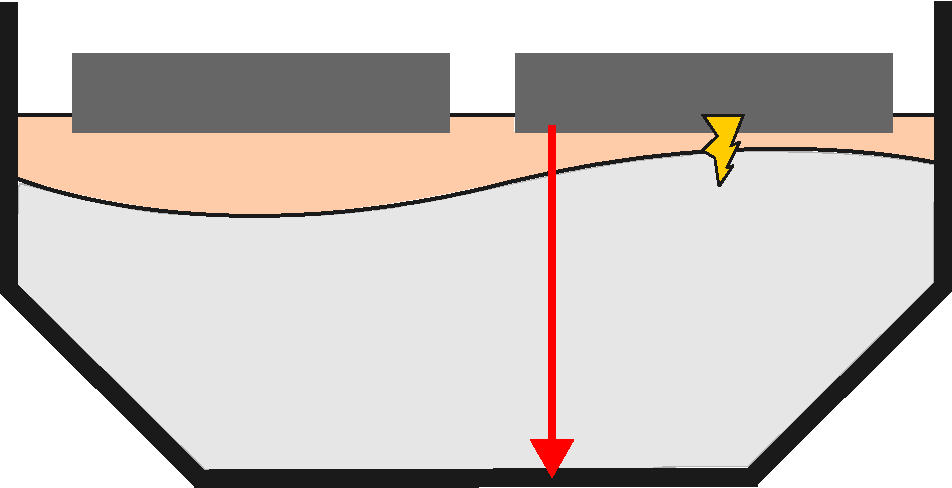
\includegraphics[height=3.5cm]{figures/intro_a.pdf}};
	\node (txt1) at (-1.5,0.5) {cryolite};
	\node (txt2) [below of=txt1, yshift=-0.1cm] {aluminum};
	\node (txt3) at (1.3,-0.7) {electrical};
	\node [below of=txt3, yshift=0.7cm] {current};
	\draw (-1.5,1.3) -- (-1,1.7) node [right] {carbon anodes} (1.27,1.7) -- (1.77,1.3);
	\node at (2.2,0.5) {risk};
\end{scope}
\begin{scope}[xshift=4cm]
	\node (pic1) at (0,0) {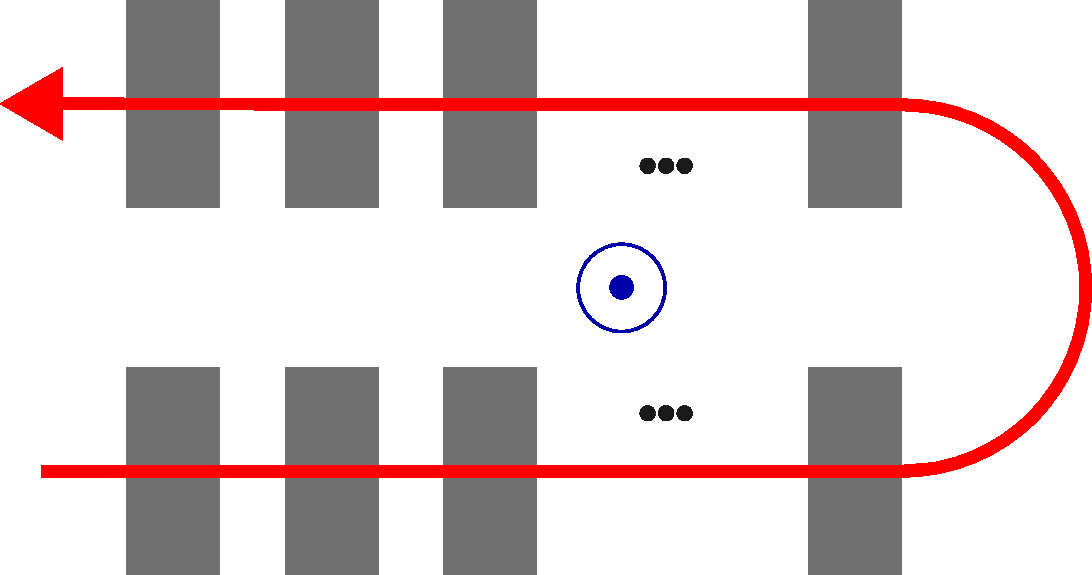
\includegraphics[height=3.5cm]{figures/intro_b.pdf}};
	\node at (2.7,1.3) {$I_0$};
	\node at (1,-0.05) {$B_z$};
\end{scope}
\node (a) at (-7.3,2) {$(a)$};
\node (b) at (1,2) {$(b$)};
\end{tikzpicture}
\caption{(a) Sideview of an aluminium reduction cell (ARC) with two superposed liquid layers. Metal pad roll instability destabilises waves on the interface and can cause short-circuits. (b) ARC's are typically arranged around a central current loop in an industrial hall and this creates an ambient magnetic field $B_z$ of typically a few mT. \label{fig:intro_fig}}
\end{figure}
%%%%%%%%%%%%%%%
In terms of hydrodynamics, ARCs can be regarded as stably stratified systems of two liquid layers carrying a strong vertical electric current, see Fig.\,\ref{fig:intro_fig}\hyperref[fig:intro_fig]{(a)}. The alumina is dissolved in molten cryolite (${\rm Na}_3{\rm Al}{\rm F}_6$) and floats  on top of a layer of reduced pure aluminum. The interface between both layers can be destabilized and set in motion by Lorentz forces, interactions between the electrical currents in the cell, and induced or external magnetic fields. Many studies have shown that the most critical instability results from the interaction of horizontal electrical  currents in the aluminum layer and the vertical component of an external magnetic field ($B_z$ in the figure) \cite[chapter~6.1]{gerbeau2006a}. As illustrated in Fig.\,\ref{fig:intro_fig}\hyperref[fig:intro_fig]{(b)}, external  magnetic fields are induced  by the power supply lines in the aluminium factory and cannot be avoided during operation. In this paper, we use the term MPR instability to refer to this particular scenario, in line with the majority of the literature. The MPR instability causes a rotating sloshing motion in the aluminum (metal pad) that must be strictly controlled throughout the electrolysis. As suggested in Fig.\,\ref{fig:intro_fig}\hyperref[fig:intro_fig]{(a)}, the cells can be short-circuited if the liquid aluminum layer makes contact with the upper carbon anodes. This causes significant damage to these anodes and is best avoided. For ARCs to remain stable with respect to the MPR-instability, the cryolite layer must not be thinner than about $3.5$\textendash$4.5\,{\rm cm}$ \cite{seetharaman2024}. This is, however, very energetically unfavorable as important Ohmic losses occur in the poorly conducting cryolite. About $40\,\%$ of a cell’s electrical energy reduces no aluminum, but is converted into waste heat. Keeping in mind that aluminum production consumes around $8\,\%$ of the global industrial electricity \cite{Kermeli2015}, the importance of understanding and controlling MPR instability is evident.
\\
\indent The first successful attempts to explain the MPR instability mechanism go back to the studies of \citet{Urata1985} and \citet{Sele1977}. On the basis of some heuristic arguments, Sele succeeded in deducing an essential non-dimensional parameter that controls the stability
\begin{align}
	\beta_{\rm S} = \frac{I_0 B_z}{(\rho_{\rm a} - \rho_{\rm c})gh_{\rm a}h_{\rm c}},
\end{align}
today referred to as the Sele parameter. In this parameter, $I_0$ and $B_z$ denote the total cell current and the vertical magnetic field, $g$ is gravity and $\rho_{\rm a}, \rho_{\rm c}$ and $h_{\rm a},h_{\rm c}$ refer to the densities and heights of the aluminum and cryolite layers. According to Sele, ARCs are MPR unstable when $\beta_{\rm S}$ exceeds a critical value, $\beta_{\rm crit}$, which depends on the lateral cell geometry, but also on the viscous or turbulent damping. The scaling behavior $\beta_{\rm S} \sim 1/h_{\rm c}$ explains why we need a thick enough cryolite layer.
\\
\indent Much progress in the theoretical modelling of the MPR instability was made in the 1990s \cite{Sneyd1994, Bojarevics1994, Davidson1998}. Perturbation techniques were applied to study the linear stability in the framework of the shallow-water approximation. It was revealed that the Lorentz force can couple different standing gravity wave modes and destabilise them by pairs, much like in a parametric resonance of waves. The MPR instability  is triggered when the natural frequencies $\omega$ and $\omega'$ of at least two transverse gravity wave modes are sufficiently close to one another. The effect of the magnetohydrodynamic coupling is that $\omega$ and $\omega'$ are shifted towards each other for increasing $I_0 B_z$ until they coincide at $\beta_{\rm S} = \beta_{\rm crit}$. If $I_0 B_z$ is further increased ($\beta_{\rm S} > \beta_{\rm crit}$), the wave-pair becomes unstable and grows exponentially to become a rotating metal pad wave. The stability threshold $\beta_{\rm crit}$ scales with the difference between the squared eigenfrequencies $\beta_{\rm crit} \sim |\omega^2 - \omega'^{2}|$ \cite{Davidson1998}. Cells in which pairs of gravity waves with identical natural frequencies $\omega = \omega'$ exist (e.g., this is the case for square and cylindrical cell geometries) are always unstable in the inviscid limit; the stability threshold in such cells only depends on the viscous or turbulent damping. An alternative view on the origin of the MPR instability was given by \citet{Lukyanov2001}, who argued that the instability is the result of multiple self-amplifying wave reflections on the sidewalls. According to \citet{Lukyanov2001}, the MHD coupling mechanism is inherently connected to the lateral walls, explaining the vocabulary of \textit{wall modes} introduced by \citet{Molokov2011}. In the decade that followed, most attention went to the development of nonlinear numerical models \cite{Zikanov2000,Zikanov2004,Bojarevics2006,gerbeau2006a} that can describe wave dynamics well beyond the stability threshold, e.g., for estimating saturation amplitudes. This has allowed ARC modeling to reach a certain level of maturity, and a great deal of effort has gone into the optimization of magnetic field and electric current distributions \cite{bojarevics2015} to maximally avoid the MPR-instability. 
\\
\indent Realizing well-controlled experiments on MPR instability in ARCs is difficult due to the high temperature ($\sim 1000^o$C) and chemical aggressiveness. For this reason, several attempts have been made to develop downscaled model experiments that can synthesize or imitate MPR waves under ambient conditions. The pioneering experiment was devised by \citet{Pedcenko2009,Pedcenko2017}, who replaced the cryolite layer with a grid of vertical thin rods imitating its electrical role. The aluminum layer was replaced by the eutectic alloy GaInSn that is liquid at room temperature. The experiment succeeded in demonstrating the MPR instability under a high imposed magnetic field, but also suffered some limitations. The steel rods were quite intrusive, and the instability was artificially intensified when the GaInSn detached from them  under wave motion. This experiment can also not be employed as a benchmark for MPR theories that suppose two fluid layers. At this point, we would like to take the opportunity to highlight that  another very sophisticated MPR experiment has been done using two immiscible transparent solutions of nitric acid ($\rm{HNO}_{\rm{3(aq)}}$ at the bottom and $\rm{HNO}_{3}$ + ${\rm C}_5\rm{H}_{12}\rm{O}$ at the top). Unfortunately, this work of \citet{Borisov2010} has only been published in a Russian-language journal, and therefore it has been overlooked.  In this set-up, both liquids have very similar densities, and the interface can be destabilized with comparatively small currents and weak magnetic fields. This is the only study that has ever reported experimental stability onsets, including the associated most unstable wave pairs as a function of the lateral aspect ratio of the cell. A similar two-layer setup using Ga-Hg liquid metal pairs was proposed \cite{Nore2021}, but no experiment has been done yet.  
\\
\indent Recently, \citet{Hegde2025} have proposed a new small-scale MPR experiment that works with one liquid layer of GaInSn. The MPR instability is synthesized through a feedback loop control that injects horizontal electrical currents  in the GaInSn-layer, proportional to the measured slope. This imitates the physics of the Sele-mechanism, but the feedback mechanism still needs to be carefully calibrated to imitate the MPR physics of two-layer cells. Another recent experiment is that of \citet{Eltishchev2022,Eltishchev2024}, who destabilized rotating surface waves through a MHD forcing mechanism that is quite similar to that of the MPR instability.
\\
\indent Spurred on by these recent experimental advances and the rediscovery of Borisov's experiment, we present here a linear stability theory that is specially dedicated to MPR instability in small-scale experimental models. In small-scale set-ups, we must account for physical ingredients that are usually neglected in ARCs, and this requires a specific theory. We can have non-shallow laters, significant viscous damping, possibly magnetic damping (for high $B_z$), and low differences in electrical conductivity between the two liquid layers, where \citet{Herreman2019} proposed a linear stability theory for small cylindrical cells, we present here a similar theory for small, rectangular cells. A perturbative approach was also used in \citet{Politis2021}, but wave-damping there was modeled in a phenomenological way. In this study, we propose a laminar viscous damping model that has no adjustable parameters and can also be compared to previous work on viscous damping of waves in two-layer systems, \cite{Keulegan1959}  and \cite{LaRocca2002}. A linear stability model consisting of equations for the growth rate and the viscous damping rate will be essential in benchmarking numerical solvers and existing MPR experiments, as well as for developing new ones. 
\\
\indent The manuscript is organized as follows: In Sec.\,\ref{sec:lsa} we calculate the growth rate of the MPR instability in small cells using  perturbation methods and including a model for viscous dissipation. In Sec.\,\ref{sec:results}, we  validate our new two-layer damping formula numerically with the DNS multiphase code ARCHER \cite{Menard2007, Vaudor2017}, and we also compare our damping rates to the experimental and numerical results of \citet{LaRocca2002}. We then calculate theoretically predicted onsets of stability as a function of cell geometry and compare with the theory of \citet{Politis2021}. We also apply our stability theory to the two-layer experimental set-up of \citet{Borisov2010}. In Sec.\,\ref{sec:discuss} we collate our results and discuss open questions.

\section{Linear stability analysis}
\label{sec:lsa}
\subsection{Formulation of the problem}

We consider a system of two superposed immiscible, incompressible and Newtonian liquid layers ($\Omega_1$ and $\Omega_2$) at rest in a rectangular domain ($x$, $y$, $z$) of dimensions $L_x$, $L_y$ and $H=h_1+h_2$. For both layers, the density $\rho_i$, kinematic viscosity $\nu_i$ and electrical conductivity $\sigma_i$ are taken into account. The subscripts $i=1,2$ refer to the upper and lower layers respectively. The origin of the coordinate system $\mathcal{O}$ is located at the center of the interface. The rigid boundaries of each layer are denoted by $\Sigma_i$. We include interfacial tension $\gamma_{\ii{int}}$ to our model, which acts in addition to gravity $g$ as a restoring force, but neglect capillary effects at the side walls, i.e., we assume that the contact line slides freely along the side walls while maintaining a static contact angle of $90^{\circ}$. The entire cell is exposed to an external homogeneous magnetic field oriented vertically $B_z$, and gravity acts in the negative $z$ direction $\h g = -g \h e_z$. At equilibrium, both layers carry a homogeneous vertical electrical current density $J_0 = -I_0/(L_xL_y)$, where $I_0$ denotes the total cell current. The equilibrium configuration  is fully characterized by the hydrodynamic pressure $P_i = P_0 - \rho_i g z$, and the electrical potential $\Phi_i = \Phi_0 - J_0z/\sigma_i$, where $P_0$ and $\Phi_0$ are constants. The cell at equilibrium is shown in Fig.\,\ref{fig:cell_schematic}. In the perturbed state, the total current density $\h J (x,y,z,t)= J_0\h e_z + \h j_i (x,y,z,t)$ takes into account the excess currents $\h j_i$ and the total magnetic field strength $\h B (x,y,z,t)= B_z\h e_z + \h b_i(x,y,z,t)$ takes into account the induced magnetic fields $\h b_i$. The perturbed interface $\mathcal{S}$ is located at $z=\eta(x,y,t)$.

\begin{figure}
	\tdplotsetmaincoords{83}{-75}
	\begin{tikzpicture}[tdplot_main_coords, scale=1]
		\filldraw[
		fill=gray!15, line width=0.05pt,
		]      (-6,-4,0)
		-- (6,-4,0)
		-- (6,4,0)
		-- (-6,4,0)
		-- cycle;
		
		\draw [very thick] (-6,-4,-2) -- (6,-4,-2);
		\draw [very thick] (-6,4,-2) -- (6,4,-2);
		\draw [very thick] (-6,-4,-2) -- (-6,4,-2);
		\draw [very thick] (6,-4,-2) -- (6,4,-2);
		
		\draw [very thick] (-6,-4,2) -- (6,-4,2);
		\draw [very thick] (-6,4,2) -- (6,4,2);
		\draw [very thick] (-6,-4,2) -- (-6,4,2);
		\draw [very thick] (6,-4,2) -- (6,4,2);
		
		\draw [very thick, dashed] (-6,-4,0) -- (6,-4,0);
		\draw [very thick, dashed] (-6,4,0) -- (6,4,0);
		\draw [very thick, dashed] (-6,-4,0) -- (-6,4,0);
		\draw [very thick, dashed] (6,-4,0) -- (6,4,0);    
		
		
		
		\draw [very thick] (-6,-4,-2) -- (-6,-4,2);
		\draw [very thick] (-6,4,-2) -- (-6,4,2);
		\draw [very thick] (6,-4,-2) -- (6,-4,2);
		\draw [very thick] (6,4,-2) -- (6,4,2);
		
		%		\begin{scope}[canvas is xy plane at z=0]
			%			\pgflowlevelsynccm
			%			\draw [-Latex, thick] (0,0,) -- (1,0);
			%		\end{scope}
		\begin{scope}[canvas is zy plane at x=0]
			\pgflowlevelsynccm
			\draw [-Latex, thick] (0,0,) -- (1.05,0) node [left, xshift=-0.7mm, rotate=-90] {\large$z$};
			\draw [-Latex, thick] (0,0) -- (0,-1,) node [right, rotate=-90] {\large$x$};
			\draw [-Latex, thick] (0,0) -- (0.4,-0.7) node [above, xshift=-2mm, yshift=-1mm, rotate=-90] {\large $y$};
			
			\draw [-Stealth, very thick] (1.05,1) -- (0,1) node [below,rotate=-90] {\Large $J_0$};
		\end{scope}
		
		\begin{scope}[canvas is zy plane at x=-6]
			%			\pgflowlevelsynccm %transforms arrows (alternative to transform shape as well)
			\draw [thick, |-|] (0,4.3) -- (2,4.3) node [left, xshift=-1cm, rotate=-90, transform shape] {\large $h_1$};
			\draw [thick, |-|] (0,4.3) -- (-2,4.3) node [left, xshift=1cm, rotate=-90, transform shape] {\large $h_2$};
			\draw [thick, |-|] (-2.3,-4) -- (-2.3,4) node [below, yshift=-4cm, rotate=-90, transform shape] {\large $L_x$};
			\node at (0,0) [right, xshift=-1.9cm, yshift=-5.5cm, rotate=-90, transform shape]{\large $L_y$};
		\end{scope}
		
		\begin{scope}[canvas is xz plane at y=-4]
			\pgflowlevelsynccm 
			\draw [thick, |-|] (-6,-2.3) -- (6,-2.3);
		\end{scope}
		
		\node (t1) at (0,0,2) {$\Omega_1(\rho_1, \nu_1, \sigma_1)$};
		\node (t2) at (0,0,-2) {$\Omega_2(\rho_2, \nu_2, \sigma_2)$};
		\node (t3) at (0,-4.65,-0.1) {$\mathcal{S}$};
		
		\node (t4) at (0,4,-1.1) {$\gamma_{\ii{int}}$};
		\node (t5) at (-4,-4.65,1.7) {$\Sigma_1$}; 
		\node [below of=t5, yshift=-25] {$\Sigma_2$};
		
		\draw [-Stealth, very thick] (0,-6.1,-0.4) -- (0,-6.1,1.6) node [above] {$B_z$};
		\draw [-Stealth, very thick] (0,-6.7,1.6) -- (0,-6.7,-0.4) node [below] {$g$};
	\end{tikzpicture}
	\caption{Schematic of the cell at equilibrium consisting of two fluid mediums $\Omega_1$ (upper), $\Omega_2$(lower) characterized by their densities $\rho_1,\rho_2$, kinematic viscosities $\nu_1,\nu_2$\textcolor{green}{,} electrical conductivity $\sigma_1,\sigma_2$,  thicknesses $h_1$,$h_2$ and bounded by rigid boundaries (container walls) $\Sigma_1$,$\Sigma_2$ respectively. Gravity $g$ acts in the negative $z$ direction, stratifying the two media with an interface $\mathcal{S}$ located at $z=0$ and characterized by interfacial tension $\gamma_{\ii{int}}$. Both layers are traversed by a homogeneous vertical electrical current density $J_0$ and submitted to a homogeneous vertical magnetic field $B_z$.}
	\label{fig:cell_schematic}
\end{figure}

\subsection{Governing equations and boundary conditions}
The perturbed quantities $(\h u_i, p_i, \h j_i, \varphi_i, \h b_i)$, for the velocity, pressure, current density, electrical potential, and induced magnetic field which modify the equilibrium state, are governed by the following equations
%%%%%%%%%%%%%%%%%%%%
\begin{subequations}
	\begin{align}
		\rho_i \partial_t{\h u}_i + {\nabla}p_i
		&= \h j_i \times \h B + \rho_i\nu_i\nabla^2\h u_i, \label{eq:gov_momentum}
		\\
		\bm{\nabla} \cdot \h{u}_i &= 0, \label{eq:gov_cont}
		\\
		\bm\nabla \cdot \h j_i &= 0,  \label{eq:charge_cont}
		\\
		\h j_i &= -\sigma_i (\bm\nabla\varphi_i + \h u_i \times \h B),
		\label{eq:gen_ohms_law}
		\\
		\bm\nabla \times \h j_i &= -\pdv{\h b_i}{t},
		\label{eq:faraday}
		\\
		\bm \nabla \times \h b_i &= \mu_0\h j_i, \qquad \bm \nabla \cdot \h b_i = 0.
		\label{eq:gauss+amp_max_law}
	\end{align} \label{eq:all_gov}
\end{subequations}
%%%%%%%%%%%%%%%%%%%%
Eq.\,\eqref{eq:gov_momentum} is the linearized conservation of momentum relation; Eq.\,\eqref{eq:gov_cont} expresses the continuity of velocity and \eqref{eq:charge_cont} the compensation current. Eq.\,\eqref{eq:gen_ohms_law} refers to the quasi-magnetostatic approximation of Ohm's law \cite{Davidson2001}. Eq.\,\eqref{eq:gen_ohms_law}, Eq.\,\eqref{eq:faraday} (Faraday's law) and Eq.\,\eqref{eq:gauss+amp_max_law}(Gauss's law) together give the following induction equation:
\begin{equation}
	\pdv{\h b_i}{t} - \bm\nabla \times (\h u_i \times \h B) - \frac{\Delta \h b_i}{\mu_0 \sigma_i},
	\label{eq:magnetic_indcution_diffusion}
\end{equation}
where $\mu_0\sigma_i$ is the magnetic diffusivity of a given material ($\mu_0$ is the permeability of free space). Eq.\,\eqref{eq:magnetic_indcution_diffusion} describes the advective and diffusive processes of the magnetic field in a given medium. Considering low magnetic field strength $\bm B$ in both layers, the Reynolds (Re), the magnetic Reynolds (R\textsubscript{m}), and magnetic Prandtl number (P\textsubscript{m}) for a given layer reads
%%%%%%%%%%%%%%%
\begin{equation}
\ii{Re} = \omega L^2/\nu, \quad
\ii{R}_{\ii m} = \mu_0\sigma \omega L^2 \ll 1, \quad \ii{P}_{\ii m} = \mu_0\sigma \nu \ll 0.01.
\end{equation} 
%%%%%%%%%%%%%%
The characteristic velocity is given as a product of the interfacial wave frequency $\omega$ and the characteristic length of the geometry $L = \sqrt{L_xL_y}$, in Potential theory. At low $\ii{R}_{\ii m}$, magnetic diffusion dominates advection and induction, and therefore, the time rate of change of magnetic field due to the liquid motion can be neglected. Furthermore, the characteristic time of diffusion is relatively smaller to all the other time scales of the flow. These two assumptions in conjunction allow us to take a static magnetic field, i.e., the  $\partial\h B/\partial t = \h u \times \h B= 0$. This assumption reduces the magnetic problem to a static case in both the liquid layers. Therefore, we can impose a magnetostatic approximation on the system where the electric field is a dependent variable of the electric potential. We therefore introduce a new dimensionless number, the magnetic Fourier number (Fo\textsubscript{m}), which encapsulates the conditions set by the previously mentioned numbers. It is given as follows:
\begin{equation}
	\ii{Fo}_{\ii m} = \frac{1}{\ii{Re} \;\ii{P}_{\ii m}} = \frac{1}{\mu_0\sigma \omega L^2}.
	\label{eq:fourier_num}
\end{equation}
 From Eq.\,\eqref{eq:fourier_num}, we can infer that the Reynolds number should be small enough to remain in the laminar regime, yet large enough for the Fourier number to be applicable in the magnetostatic approximation. Though we state the system of equations consisting of the induced magnetic field perturbation $\h b_i$ in Eq.\,\eqref{eq:gauss+amp_max_law}, it is of no importance in this study. Previous studies based on shallow water theories have largely ignored the contribution of the induced magnetic field on the perturbed Lorentz force \citep{Bojarevics1994, Davidson1998}. In a cylindrical system, it was shown that $\h J \times \h b_i$ does not contribute to the amplitude of the wave but rather to the frequency shift \citep{Herreman2019}. This is because the Lorentz force due to the horizontal component of the induced magnetic field $\h J \times \h b_i$ is out of phase with $\h J \times B_z\h e_z$ (the dominant contribution) and therefore, cannot inject power into the wave.
\\
\indent For the formulation of the boundary conditions at the tank walls, we account for the fact that the upper carbon anode in ARCs is a much better electrical conductor than the cryolite, and the bottom steel cathode often a much poorer conductor than aluminum. For this idealized case, in which excess currents close entirely in the aluminum layer, we obtain the following linearized boundary conditions:
%%%%%%%%%%%%%%%%%%%%
\begin{subequations}
	\begin{align}
		\bm{j}_1\cdot \h e_x\bigl|_{x=-L_x/2} &= \bm{j}_2\cdot \h e_x\bigl|_{x=L_x/2} = 0,  \label{eq:bc1}
		\\
		\h j_1\cdot \h e_y\bigl|_{y=-L_y/2} &= \h j_2\cdot \h e_y\bigl|_{y=L_y/2} = 0,  \label{eq:bc2}
		\\
		\varphi_1 &= 0 \,\bigl|_{z=h_1}, \label{eq:bc3}
		\\
		\h j_2\cdot \h e_z &= 0\,\bigl|_{z=-h_2} . \label{eq:bc4}
	\end{align} 
\end{subequations}
%%%%%%%%%%%%%%%%%%%%
Eqs.\,\eqref{eq:bc1} and \eqref{eq:bc2} ensure that no current can escape through the insulating side walls. The anode is modeled as an iso-potential surface [Eq.\,\eqref{eq:bc3}] and the weakly conducting cathode is treated as a perfect insulator [Eq.\,\eqref{eq:bc4}] for the excess current component $\h j$. In Sec.\,\ref{sec:Borisov}, we further consider a case where the cathode is modeled as a perfect conductor, in that respect, condition [Eq.\,\eqref{eq:bc4}] is not valid for all reduction cells and MPR model experiments. As for the kinematic boundary conditions, we simply apply  impermeability at all walls
\begin{equation}
	\h u_i \cdot \h n_i|_{\Sigma_i} = 0,
	\label{eq:no-outflow_bc}
\end{equation}
for the inviscid formulation (no slip condition) in Sec.\,\ref{sec:Ansatz} to which we must add
\begin{equation}
	\h u_i \times \h n_i|_{\Sigma_i} = 0.
\end{equation}
to account for viscous effects, we address in Sec.\,\ref{sec:visc_damp}. At the interface $\mathcal{S}$, we have to take into account the following linearized  hydrodynamic and electrical boundary conditions:
%%%%%%%%%%%%%%%%%%%%
\begin{subequations}
	\begin{align}
		\partial_t \eta &= u_{1,z} \,\bigl|_{z = 0} = u_{2,z} \bigl|_{z = 0},  \label{eq:int_bc1}
		\\
		-\gamma_{\ii{int}} \nabla^2\eta + (\rho_2-\rho_1)g\eta &= p_2 \,\bigl|_{z=0} - p_1 \,\bigl|_{z=0},  \label{eq:int_bc2}
		\\
		\h	j_1 \cdot \h e_z &= \h j_2\cdot \h e_z \,\bigl|_{z = 0}, \label{eq:int_bc3}
		\\
		J_0(\sigma_1 - \sigma_2)\eta &= \varphi_2 \,\bigl|_{z=0} -\varphi_1 \,\bigl|_{z=0}. \label{eq:int_bc4}
	\end{align}
\end{subequations}
%%%%%%%%%%%%%%%%%%%%
Eqs.\,\eqref{eq:int_bc1} and \eqref{eq:int_bc2} represent the classic kinematic and dynamic boundary conditions for gravity-capillary waves. In Sec.\,\ref{sec:visc_damp}, we state the corrections to Eq.\eqref{eq:int_bc2} incorporating the continuity of the tangential velocities and viscous stresses in order to solve the Stokes velocities (for viscous damping). The electrical boundary conditions are derived from the basic principle that both the normal of the total current density $\h n \cdot \h J$ and the total electric potential $(\Phi_i+\varphi_i)$ must remain continuous. This results in the linearized interfacial conditions [Eq.\,\eqref{eq:int_bc3}] and [Eq.\,\eqref{eq:int_bc4}] for the perturbed quantities \citep{Munger2006}. This jump condition is essential for the MPR instability as it describes how the current density redistributes in both layers as a response to an arbitrary (small) interface elevation $\eta$. Because the horizontal component of the redistributed current is responsible for the Lorentz force that reinforces interface displacements $\eta$, the self-destabilization is mainly anchored in this interfacial boundary condition. 


\subsection{Two-wave perturbation approach}
\label{sec:Ansatz}
The perturbative approach is based on the (inviscid) potential flow solutions of free gravity-capillary interfacial waves that form a set of orthogonal functions in the absence of MHD effects ($\bm{B},\bm{J}= \bm 0$) and without viscosity ($\nu = 0$). Viscosity only affects the flow in the close vicinity of the Stokes boundary layers forming at the container walls, and below and above the interface. In Sec.\,\ref{sec:visc_damp}, we calculate Stokes boundary layers corrections to the potential flow solutions to predict viscous damping rates associated with interfacial wave motions. In our formulation, however, only perturbations of the inviscid bulk flow are considered and all dissipative effects are integrated into a global damping factor $\lambda$. In contrast to most previous studies, which examine the interaction of infinitely many wave modes and truncate the system \textit{a posteriori} \cite{Sneyd1994,Bojarevics1994}, we calculate the two-wave interaction directly allowing us to derive exact analytical solutions for the growth rates and stability onsets. The disadvantage of this method is that the MPR instability can sometimes arise from three (or more)-wave interactions. Accordingly, these cases are not represented in our model. As a final presumption, we suppose that both waves are magnetohydrodynamically coupled within their base state and therefore both oscillate with the same mean frequency. We represent the average natural frequency of the wave as $\bar{\omega} = (\omega + \omega')/2$ and attenuation with the mean damping rate as $\bar{\lambda} = (\lambda + \lambda')/2$. Similarly, the average frequency difference as $\delta\omega = (\omega - \omega')/2$ and decay rate difference as $\delta{\lambda} = (\lambda - \lambda')/2$.   In light of these assumptions, we propose the following two-wave ansatz:
%%%%%%%%%%%%%%%%
\begin{equation}
	\fontsize{10.5pt}{10.5pt}
	[\textbf{\textit{u}}_i, p_i, \eta, \textbf{\textit{j}}_i ]= 
	\biggl( 
	C 
	\left[ 
	\widehat{\h{u}}_{i}, \widehat{p}_{i}, \widehat{\eta}, \widehat{\h{j}}_{i} \right] 
	+ 
	C' 
	\left[ 
	\widehat{\h{u}}'_{i}, \widehat{p}'_{i}, \widehat{\eta}', \widehat{\h{j}}'_{i} \right] 
	+\left[
	\widetilde{\h{u}}_i, \widetilde{p}_{i}, \widetilde{\eta}, \widetilde{\h{j}}_{i} \right] 
	\biggr) 
	\;
	\ii e^{ \bigl(\alpha -\overbar\lambda 
		\,+\, \ii{i}\overbar{\omega}
		\bigr)t} .
	\label{eq:perturb_method_ansatz}
\end{equation}
%%%%%%%%%%%%%%%%%%%%

In this notation, the tilded variables are small perturbations with respect to the hatted variables representing the basic two-wave state. The eigenvalues $C$ and $C'$ are to be determined and $\alpha$ is the potentially destabilizing contribution to the growth rate that we seek to derive. The wave pair is MPR unstable if and only if $\alpha$ is both a real number and exceeding the mean damping rate $\alpha > \bar{\lambda}$. The total growth rate $\alpha_{\rm MPR}$ is then given by the difference $\alpha_{\rm MPR} = \alpha - \bar{\lambda}$ and stability onsets are defined by the condition $\alpha = \bar{\lambda}$. Considering the wave pair to be in a coupled motion $\omega = \omega' = \bar{\omega}$ is justified by the fact that the wave frequencies are shifted by Lorentz forces ($\bar{\omega} = \omega - \delta \omega$ and $\bar{\omega} = \omega' + \delta \omega$) in such a way that they coincide exactly at the point of marginal stability \cite{Davidson1998}. In the absence of any Lorentz forces, precisely the classic gravity-capillary wave modes given in Eq.\,(\ref{eq:perturb_method_ansatz}) result as two independent solutions of our system. This rigorously justifies our approach, and our theory is capable of describing the complete transition from purely hydrodynamic waves passing through magnetohydrodynamically modified waves regimes up to the (linear) self-amplifying MPR wave.
\\
\indent To formulate the base state, we assign the hatted quantities with the classical gravity-capillary wave solutions that can be obtained by expressing the bulk velocities as gradients of scalar potentials $\widehat{\h u}_i = \bm\nabla \widehat\phi_i$ and solving the Laplace equation $\bm\nabla^2\widehat\phi_i = 0$ together with the no outflow boundary condition [Eq.\,\eqref{eq:no-outflow_bc}] and the interface conditions given in Eqs.\,\eqref{eq:int_bc1} and \eqref{eq:int_bc2}. The linear inviscid solutions for perturbation quantities of a singular wave mode ($m,n$) can be represented as follows:
%%%%%%%%%%%%%%%%%%%%
\begin{equation}
	\begin{bmatrix}
		\widehat{\h u}_i \\[5pt]
		\widehat{p}_i \\[5pt]
		\widehat{\eta}
	\end{bmatrix}
	=
	\begin{bmatrix}
		\bm{\nabla}\widehat{\phi}_i \\[5pt]
		-\rho_i(\ii i\omega)\widehat{\phi}_i\\[5pt]
		\partial_z \widehat{\phi}_i/(\ii i\omega )
	\end{bmatrix},
	\label{eq:pot_wave_soln}
\end{equation}
%%%%%%%%%%%%%%%%%%%%
with the leading-order flow potentials given as
%%%%%%%%%%%%%%%%%%%%
\begin{equation}
	\begin{bmatrix}
		\widehat{\phi}_{1} \\[12pt]
		\widehat{\phi}_{2} 
	\end{bmatrix} = 
	A_{mn}
	\left[
	\begin{array}{cc}
		\dfrac{\omega}{k} \dfrac{\cosh[k(z-h_1)]}{\sinh[k h_1]} & 
		\\[10pt]
		-\dfrac{\omega}{k} \dfrac{\cosh[k(z+h_2)]}{\sinh[k h_2]} &
	\end{array} 
	\right] 
	\cos\left[\dfrac{m\pi}{L_x}\left( x + \dfrac{L_x}{2} \right)\right]
	\cos\left[\dfrac{n\pi}{L_y}\left( y + \dfrac{L_y}{2} \right)\right]
	\label{eq:vel_potential}
\end{equation}
%%%%%%%%%%%%%%%%%%%%
along with the interface elevation function reading
\begin{equation}
	\widehat\eta = \ii{i}\,A_{mn} \cos\left[\dfrac{m\pi}{L_x}\left( x + \dfrac{L_x}{2} \right)\right]
	\cos\left[\dfrac{n\pi}{L_y}\left( y + \dfrac{L_y}{2} \right)\right] .
	\label{eq:eta_eq}
\end{equation} 
%%%%%%%%%%%%%%%
Here, $A_{mn}$ are mode-dependent wave amplitudes, $k$ is a function of the wave numbers $(m,n) \in \mathbb{N}^{0}\times\mathbb{N}^{0}$
%%%%%%%%%%%%%%%
\begin{equation}
	k =  \pi\sqrt{\frac{m^2}{L_x^2} + \frac{n^2}{L_y^2} }\,
\end{equation}
%%%%%%%%%%%%%
and the natural frequencies of the gravity-capillary waves are obtained as
%%%%%%%%%%%%%%%%%%%%
\begin{equation}
	\omega = \pm \sqrt{
		\dfrac{(\rho_2-\rho_1)gk + \gamma_{\scaleto{\ii{int}}{5pt}}{k}^3}
		{\rho_1 \coth[k\: h_1]
			+ \rho_2 \coth[k\: h_2]}
	} \,.
	\label{eq:omega}
\end{equation}
%%%%%%%%%%%%%%%%%%%%
We retrieve the classical dispersion relation obtained by \citet{mikaelian1990} in the context of Rayleigh-Taylor instabilities. The sign associated with $\omega$ plays an important role in determining the nature of instability. Wave motions in alignment with the direction of the Lorentz forces tend to amplify, whereas those in the opposite direction tend to dampen. 
\\
\indent It remains to calculate the leading-order current perturbations through Ohm's law $\widehat{\h j}_i = -\sigma_i\bm\nabla \widehat\varphi_i$. The electric potentials must also fulfill the Laplace equation $\bm{\nabla}^2\widehat{\varphi} = 0$ with boundary conditions given in Eqs.\,(\ref{eq:bc1} -- \ref{eq:bc4}), \eqref{eq:int_bc3} and \eqref{eq:int_bc4}. As the electrical boundary conditions at the insulating side walls are identical to the hydrodynamic outflow condition [Eq.\,\eqref{eq:no-outflow_bc}], the solutions of $\widehat\varphi_i$ result in a very similar form:
%%%%%%%%%%%%%%%%%%%%
\begin{equation}
	\begin{bmatrix}
		\widehat{\varphi}_1 \\[12pt]
		\widehat{\varphi}_2 
	\end{bmatrix} = 
	J_0\,\Lambda\,\widehat{\eta}
	\left[
	\begin{array}{cc}
		-\dfrac{\sinh[k (z-h_1)]}{\sigma_1 \cosh[kh_1]} &
		\\[10pt]
		-\dfrac{\cosh[k (z+h_2)]}{\sigma_2 \sinh[kh_2]} & 
	\end{array} 
	\right] ,
	\label{eq:elec_potential}
\end{equation}
%%%%%%%%%%%%%%%%%%%%
where $\Lambda$ can be referred to as the conductivity-jump parameter reading
%%%%%%%%%%%%%%%%%%%%
\begin{equation}
	\Lambda = \frac{(\sigma_1^{-1} - \sigma_2^{-1})}{\sigma_1^{-1} \:\tanh[kh_1] + \sigma_2^{-1} \:\coth[kh_2]} .
\end{equation}
%%%%%%%%%%%%%%%%%%%%

\subsection{Calculation of the growth rate}
\label{sec:growth_rate_gen}
All the preparations have now been made to calculate the growth rate $\alpha_{\ii {MPR}}$. By inserting the ansatz [Eq.\,\eqref{eq:perturb_method_ansatz}] in the governing Eqs.\,\eqref{eq:gov_momentum} and \eqref{eq:gov_cont}, and considering only the leading order terms, we can obtain the next order in the perturbation problem through the equations:
%%%%%%%%%%%%%%%%%%%%
\begin{subequations}
	\begin{align}
		\nn
			C&(\ii{i}\overbar\omega - \overbar\lambda + \alpha)\rho \widehat{\h{u}} + C\bm{\nabla}\widehat{p} 
			+ C'(\ii{i}\overbar\omega - \overbar\lambda + \alpha)\rho\widehat{\h{u}}' 
			+ C'\bm{\nabla}\widehat{p}'
			+ (\ii{i}\overbar\omega - \overbar\lambda) \rho\widetilde{\h{u}} 
			+ \bm{\nabla}\widetilde{p}
			\\
			+ &(\ii{i}\overbar\omega - \overbar\lambda) \rho\widetilde{\h{u}}' 
			+ \bm{\nabla}\widetilde{p}'
			= C \left( \; \widehat{\h{j}} \times B_z\bm{e}_z\right) 
			+ 
			C' \left( \; \widehat{\h{j}}' \times B_z\bm{e}_z\right)
		 ,
		\label{eq:momentum_fredholm}
	\end{align}
	\begin{equation}
		\bm\nabla \cdot \widetilde{\h u}_i = 0 .
		\label{eq:cont_fredholm}
	\end{equation}
\end{subequations}
%%%%%%%%%%%%%%%%%%%%
To find an equation for $\alpha$, we have to state a solvability condition. For that we apply the Fredholm alternative in an analogue manner to \citet{Herreman2019}. All technical calculations are provided in Appendix\,\ref{appA} in detail. The solvability condition results in an eigenvalue problem in form of a $2\times 2$ interaction matrix that can be expressed in the following form:
%%%%%%%%%%%%%%%%%%%%
\begin{equation}
	\begin{bmatrix}
		\dfrac{I_{\eta\eta}}{2K_{\eta\eta}} + \ii{i}\delta\omega - \delta\lambda -\alpha & \dfrac{I_{\eta\eta'}}{2K_{\eta\eta}} \\
		\\
		\dfrac{I_{\eta'\!\eta}}{2K_{\eta'\!\eta'}} & \dfrac{I_{\eta'\!\eta'}}{2K_{\eta'\!\eta'}} - \ii{i}\delta\omega + \delta\lambda -\alpha
	\end{bmatrix}
	\begin{bmatrix}
		C \\
		\\
		C'
	\end{bmatrix}
	= 0 ,
	\label{eq:alpha_matrix_initial}
\end{equation}
%%%%%%%%%%%%%%%%%%%%
with,
%%%%%%%%%%%%%%%%%%%%
\begin{subequations}
	\begin{align}
		I_{\eta\eta} &= \sum_{i=1,2}\int_{V_i} \widehat{\h u}_i^{*} \cdot 
		\Bigl( \; \widehat{\h{j}}_i \times B_z\bm{e}_z \Bigr) 
		= \sum_{i=1,2}\int_{V_i} \bm\nabla\widehat{\phi}_i^{*} \cdot 
		\Bigl( \; \sigma_i\bm\nabla\widehat{\varphi}_i \times B_z\bm{e}_z \Bigr) 
		= 0, \label{eq:A_11} \\
		I_{\eta\eta'} &= \sum_{i=1,2}\int_{V_i} \widehat{\h u}_i^{*} \cdot 
		\Bigl( \; \widehat{\h{j}}'_i \times B_z\bm{e}_z \Bigr) 
		= \sum_{i=1,2}\int_{V_i} \bm\nabla\widehat{\phi}_i^{*} \cdot 
		\Bigl( \; \sigma_i\bm\nabla\widehat{\varphi}'_i \times B_z\bm{e}_z \Bigr) ,
		\label{eq:A_12}\\
		I_{\eta'\!\eta} &= \sum_{i=1,2}\int_{V_i} \widehat{\h u}'^{*}_i \cdot 
		\Bigl( \; \widehat{\h{j}}_i \times B_z\bm{e}_z \Bigr) 
		= \sum_{i=1,2}\int_{V_i} \bm\nabla\widehat{\phi}'^{*}_i \cdot 
		\Bigl( \; \sigma_i\bm\nabla\widehat{\varphi_i} \times B_z\bm{e}_z \Bigr) ,
		\label{eq:A_21}\\
		I_{\eta'\!\eta'} &= \sum_{i=1,2}\int_{V_i} \widehat{\h u}'^{*}_i \cdot 
		\Bigl( \; \widehat{\h{j}}'_i \times B_z\bm{e}_z \Bigr)
		= \sum_{i=1,2}\int_{V_i} \bm\nabla\widehat{\phi}'^{*}_i \cdot 
		\Bigl( \; \sigma_i\bm\nabla\widehat{\varphi}'_i \times B_z\bm{e}_z \Bigr)
		= 0 . \label{eq:A_22}
	\end{align}
\end{subequations}
%%%%%%%%%%%%%%%%%%%%
The terms given above are associated with the power that can be injected by Lorentz forces. Eqs.\,\eqref{eq:A_11} and \eqref{eq:A_22} describe the interaction of the wave modes $\eta$ and $\eta'$ with their self-induced Lorentz forces. However, these integrals disappear, which explains why standing waves cannot be destabilized. The terms $K_{\eta\eta}$ is associated with the potential (or equivalently kinetic) energy of the respective wave modes $(m,n)$ and is given by
%%%%%%%%%%%%%%%%%%%%
\begin{align}
	\nn
	K_{\eta\eta} &= \int_{\mathcal{S}} \Bigl( -\gamma_{\ii{int}} |\bm{\nabla}\widehat{\eta}|^2 
	+ (\rho_2 - \rho_1)g |\widehat{\eta}|^2 \Bigr)\Bigl|_{z=0} \ii{d}S  ,
	\\
	& = \xi_{m\times n} \: L_xL_y \: \Bigl[\gamma_{\ii{int}}k^2 + (\rho_2 - \rho_1)g \Bigr] ,
	\label{eq:K_11}
\end{align}
Similarly, $K_{\eta\eta}$ is a function of $(m',n')$ and $k'$. For the sake of simplicity, we introduced an auxiliary function $\xi_r$ that is defined as follows
\[
\xi_r = \biggl\{
\begin{array}{c}
	1/2 , \quad r = 0  \\
	1/4 , \quad r \neq 0
\end{array} .
\]
%%%%%%%%%%%%%%%%%%%%
Finally, the secular equation of the matrix [Eq.\,\eqref{eq:alpha_matrix_initial}] yields the solutions for $\alpha$
%%%%%%%%%%
\begin{equation}
	\alpha = \pm \; \sqrt{\dfrac{I_{\eta\eta'}I_{\eta'\!\eta}}{4K_{\eta\eta}K_{\eta'\!\eta'}} + \bigl[ \ii i{\delta \omega} -\delta\lambda \bigr]^2 }.
\end{equation}
%%%%%%%%%%%%%%%%%%%%
By subtracting the damping rate $\overbar\lambda$ and solving the integrals in Eqs.\,\eqref{eq:A_12} and \eqref{eq:A_21}, we obtain the MPR growth rate, the central result of our study, that can be represented as follows
%%%%%%%%%%%%%%%
\begin{equation}
	\alpha_{\ii {MPR}} = \alpha - \overbar\lambda
	= \pm \; 
	\sqrt{ J^2{B_z}^2{\Theta}^2
		\; (\overbar\omega^2 - \delta\omega^2)
		\;\frac{\mathcal{T}\mathcal{T}'}{\mathcal{U}\mathcal{U}'}
		+ \bigl[ \ii i{\delta \omega} -\delta\lambda \bigr]^2
	} \;-\; \overbar\lambda ,
	\label{eq:main_gr}
\end{equation}
%%%%%%%%%%%%%%%%%%%%
where 
%%%%%%%%%%%%%%%%%%%%
\begin{subequations}
	\begin{gather}
		\Theta = \pm \; \sqrt{\delta_{m \times m'}\;\delta_{n \times n'}} \; 
		\frac{((-1)^{m+m'}-1)((-1)^{n+n'}-1)(m^2{n'}^2 - {m'}^2n^2)}
		{(m^2 - {m'}^2)(n^2 - {n'}^2) },
		\label{eq:form_function}
		\\
		\delta_r = \left\{ \begin{array}{cc}
			1, & r=0\\
			2, & r>0
		\end{array} \right. \!\!.
		\label{eq:delta_func}
		\intertext{The term $\Theta$ here defines the wave mode selection function, which is nonzero only if $m+m'$ and $n+n'$ are both odd, and}
		\mathcal{U} = L_xL_y\Bigl(\gamma_{\ii{int}} \: k^2 + (\rho_2 - \rho_1)g \Bigr), \qquad
		\mathcal{U}' = L_xL_y\Bigl(\gamma_{\ii{int}}\: {k'}^2 + (\rho_2 - \rho_1)g \Bigr) ,
		%%%%%%%%%%%%
		\intertext{are representations of the potential energy of the standing waves and}
		%%%%%%%%%%%%
		\mathcal{T} = \frac{\Lambda}{k(k^2 - k'^2)}
		\Biggl( 
		\frac{k}{\tanh[k'h_2]} - \frac{k'}{\tanh[kh_2]}
		+ \frac{k'\:\sech[k'h_1]}{\sinh[kh_1]}
		-\frac{k'}{\tanh[kh_1]}
		+ k\tanh[k'h_1] \Biggr) ,
		\label{eq:T_11}
		\\
		\mathcal{T}' = \frac{\Lambda'}{k'({k'}^2-k^2)}
		\Biggl( 
		\frac{k'}{\tanh[kh_2]} - \frac{k}{\tanh[k'h_2]}
		+ \frac{k\: \sech[kh_1]}{\sinh[k'h_1]}
		-\frac{k}{\tanh[k'h_1]}
		+ k'\tanh[kh_1] \Biggr) , 
		\label{eq:T_22}
		%%%%%%%%%%%%
		\intertext{root from the power injected by the Lorentz force and represent the non-shallow part of the formula. At the limit $k' \rightarrow k$ these terms simplify to}
		%%%%%%%%%%%%
		\mathcal{T} = \mathcal{T}' = \frac{\Lambda}{4k^2\:\sinh^2[kh_2]}
		\biggl( \frac{\sinh[k(h_1+2h_2)]}{\cosh[kh_1]} +2kh_2 - \tanh[kh_1] \biggr) .
	\end{gather}
\end{subequations}
%%%%%%%%%%%%%%%%%%%%
The perturbation analysis results in two distinct solutions for the growth rate $\alpha_{\rm MPR}$. The two solutions correspond to MPR waves that rotate either clockwise or anti-clockwise (when looking at the cell from above), or equivalently, to standing wave pairs ($\eta + \eta'$) with a positive or negative phase shift. One of the two wave solutions is always suppressed by the Lorentz force (when the induced Lorentz force $\h j\times B_z\h e_z$ opposes the rotating wave motion $\h u$) and the other one is amplified in the unstable situations (when $\h j\times B_z\h e_z$ aligns with $\h u$). In our configuration shown in Fig.\,\ref{fig:cell_schematic}, anti-clockwise rotating waves are destabilized. 
\\
\indent From the growth rate {Eq.\,\eqref{eq:main_gr}} one can readily derive the stability onset that is defined by the equivalence of the real part of the square root in [Eq.\,\eqref{eq:main_gr}] with $\overbar\lambda$. In order to find a preferably simple expression, we introduce a modified Sele parameter $\beta_{\gamma_{\ii{int}}}$, similar to \citet{Horstmann2018}, which takes into account interfacial tension in addition to gravity. In this way, the stability criterion can be represented compactly in a dimensionless form as follows
%%%%%%%%%%%%%%%%
\begin{equation}
	\beta_{\gamma_{\ii{int}}} > \beta_{\ii{crit}} =  \frac{L_x^2 L_y^2}{h_1h_2 \Theta}
	\sqrt{ \frac{\overbar\lambda^2 - \bigl[ \ii i{\delta \omega} -\delta\lambda \bigr]^2} {(\overbar\omega^2 - {\delta\omega}^2) \mathcal{T}\mathcal{T}'} },
	\quad \ii{where}\;\,
	\beta_{\gamma_{\ii{int}}} = \frac{I_0B_z}{\left[ (\rho_2-\rho_1)g + \gamma_{\ii{int}}\bar{k}^2 \right] h_1h_2} .
	\label{eq:beta_crit-onset}
\end{equation}
%%%%%%%%%%%%%%
In order to analyse the stability of large-scale aluminum reduction cells, the criterion can be further simplified. We reformulate Eq.\,\eqref{eq:beta_crit-onset} in the shallow-water limit and neglect interfacial tension. Then the interfacial waves become non-dispersive ($\omega = ck$, $\omega' = ck'$), with
%%%%%%%%%%%%%%%
\begin{equation}
	c = \sqrt{ \frac{(\rho_2 - \rho_1)g}{\rho_1/h_1 + \rho_2/h_2 } } .
	\label{eq:wave-speed}
\end{equation}
%%%%%%%%%%%%%%%
The product $\mathcal{T}\mathcal{T'}$ simplifies as
\begin{equation}
	\mathcal{T}\mathcal{T'} = \frac{1}{k^4k'^4h_1^2h_2^2},
\end{equation}
and therewith Eq.\,\eqref{eq:beta_crit-onset} reduces to
%%%%%%%%%%%%%%%
\begin{equation}
	\beta_{\ii{crit}} = \frac{L_x^2 L_y^2}{c \,\Theta}
	\sqrt{k^3k'^3 \, \left( \overbar\lambda^2 - \bigl[ \ii i{\delta \omega} -\delta\lambda \bigr]^2 \right) } .
	\label{eq:beta_crit_shallow}
\end{equation}
%%%%%%%%%%%%%%
This stability threshold criterion coincides with the solution of linear MPR instability presented in \citet{Politis2021}, see Sec.\,\ref{sec:fractal}. As a final simplification, we shall take a look at the academic case of square cells, which is physically relevant for some MPR model experiments \cite{Pedcenko2009,Borisov2010,Grants2021,Hegde2025}. For a square cell we have $L_x=L_y$ and $\lambda=\lambda'=\overbar\lambda$ and the parameters further reduce to $\Theta = 4$, $k=\pi/L$, $\delta\omega=0$, $\delta\lambda=0$, yielding
%%%%%%%%%%%%%%%
\begin{equation}
	\beta_{\ii{crit}} = \frac{\pi^3L}{4\, c}\,\lambda .
	\label{eq:beta_crit_square-shallow}
\end{equation} 
%%%%%%%%%%%%%%%  
As expected, the critical Sele parameter in this case is not dictated by the difference in natural frequencies anymore but solely by the damping parameter $\lambda$, as is true for all infinitely many inherently unstable aspect ratios, refer to Sec.\,\ref{sec:fractal}, Eq.\,(\ref{eq:fractal}).

\subsection{The viscous damping rate}
\label{sec:visc_damp}

Up to this point, we have been treating $\lambda$ as a purely phenomenological damping parameter. To evaluate the stability of industrial ARCs, in which turbulent flows usually prevail, $\lambda$ must be estimated or determined experimentally. In small-scale models, where flows remain largely laminar (at least in the boundaries or around the point of marginal instability), viscous damping rates can be calculated analytically. This is a key ingredient for our model to serve as a benchmark. We start with the viscous damping rate. In the leading order, magnetohydrodynamics effects can be neglected (no consideration of Hartmann layers) and it remains to calculate the total dissipation produced in the Stokes boundary layers, which are created solely by wave motions. We follow the approach by \citet{Keulegan1959}, who has calculated damping rates of free-surface gravity waves in rectangular containers. We extend his formulation to two liquid layers, which is not straightforward as viscous boundary layers are formed above and below the interface in two-liquid systems that do not develop on free surfaces and must be calculated separately. In absence of MHD effects, the linear governing Eqs.\,\eqref{eq:gov_momentum} and \eqref{eq:gov_cont} reduce to
%%%%%%%%%%%%
\begin{equation}
	\left.
	\begin{array}{c}
		\rho_i \partial_t \h{u}_i + \bm{\nabla}p_i = \rho_i\nu_i\nabla^2\h u_i 
		\\[5pt]
		\bm{\nabla} \cdot \h{u}_i = 0 
	\end{array}
	\right\} .
	\label{eq:visc_gov1}
\end{equation}
%%%%%%%%%%%%
For the upper and lower layer ($i=1,2$), the no slip condition at the side wall (represented as rigid boundary $\Sigma_i$) is  
%%%%%%%%%%%%
\begin{subequations}
	\begin{equation}
		\h u_i \big|_{\Sigma_i} = 0,
	\end{equation}
	%%%%%%%%%%%%%%
	and the tangential velocities (denoted by $\perp$) must be equal at the interface:
	%%%%%%%%%%%%%%%%
	\begin{equation}
		\h u_{1, \perp}\big|_\mathcal{S} = \h u_{2, \perp}\big|_\mathcal{S}.
		\label{eq:visc_bc1}
	\end{equation}
	%%%%%%%%%%%%%%
	The dynamic boundary condition [Eq.\,\eqref{eq:int_bc2}] under the consideration of viscous effects now changes to
	%%%%%%%%%%%%%%%%
	\begin{equation}
		p_2|_\mathcal{S} - p_1|_\mathcal{S} = 
		(\rho_2 -\rho_1)g\eta -\gamma_{\ii{int}}\nabla^2\eta 
		+ 2( \rho_2\nu_2\partial_z u_{2,z}  - \rho_1\nu_1\partial_z u_{2,z}), 
		\label{eq:visc_bc2}
	\end{equation}
	%%%%%%%%%%%%%%
	while the continuity of the tangential stresses are
	%%%%%%%%%%%%%%
	\begin{equation}
		\rho_1\nu_1 \Bigl( \partial_z u_{1,x} + \partial_x u_{1,z} \Bigr)\Bigl|_\mathcal{S}
		=
		\rho_2\nu_2 \Bigl( \partial_z u_{2,x} + \partial_x u_{2,z} \Bigr)\Bigl|_\mathcal{S},
		\label{eq:visc_bc3}
	\end{equation}
	\begin{equation}
		\rho_1\nu_1 \Bigl( \partial_z u_{1,y} + \partial_y u_{1,z} \Bigr)\Bigl|_\mathcal{S}
		=
		\rho_2\nu_2 \Bigl( \partial_z u_{2,y} + \partial_y u_{2,z} \Bigr)\Bigl|_\mathcal{S} .
		\label{eq:visc_bc4}
	\end{equation}
\end{subequations}
%%%%%%%%%%%%
In a stratified two-layer system, consider an interfacial gravity wave mode of $(m,n)$ of amplitude $A_{mn}$ oscillating at angular frequency $\omega$ undergoes viscous decay over time at a rate of $\lambda$. The fluid velocity taking into account the Stokes boundary layer corrections can be formulated as
%%%%%%%%%%%%
\begin{equation}
	\h u_i = C \Bigl[  \widehat{\h u}_i + \widehat{\bar{\h u}}_i
	\Bigr] e^{(\ii{i}\omega - \lambda) t} .
	\label{eq:visc_ansatz}
\end{equation}
%%%%%%%%%%%%
where the $\widehat{\h u}_i$ are the potential flow velocities and the barred term $\widehat{\bar{\h u}}_i$ are the viscous corrections to be calculated. We introduce wall-normal coordinates $\zeta$ that tend to decay the viscous boundary layer corrections to zero as they traverse inwards in the bulk. We define $\zeta$ as follows:
%%%%%%%%%%%%
\begin{equation}
	\zeta = \begin{cases}
		z - h_1, \qquad &\text{near } z=h_1 \\
		\dfrac{L_x}{2} - x, \qquad &\text{near } x = L_x/2 \\[7pt]
		\dfrac{L_y}{2} - y, \qquad &\text{near } y = L_y/2 \\
		z, \qquad &\text{near } z=0
	\end{cases}, 
	\qquad
	\zeta = \begin{cases}
		z + h_2, \qquad &\text{near } z=-h_2 \\
		x + \dfrac{L_x}{2}, \qquad &\text{near } x = -L_x/2 \\[7pt]
		y + \dfrac{L_y}{2}, \qquad &\text{near } y = -L_y/2 \\
		-z, \qquad &\text{near } z=0
	\end{cases} .
\end{equation}
%%%%%%%%%%%%%%%%
The effect of the diffusive boundary layer tends to diminish in the bulk region. Inserting the ansatz [Eq.\,\eqref{eq:visc_ansatz}] into Eq.\,\eqref{eq:visc_gov1}, we obtain $\widehat{\bar{\h u}}_i  \cdot \h n_i = 0$ and $\widehat{\overbar{p}}_i= 0$; the wall-normal boundary layer correction for velocity and leading-order boundary layer correction for pressure, both equal to zero. We compute the Stokes boundary layer at the domain walls (with no-slip condition) as
%%%%%%%%%%%%%%%
\begin{equation}
	\ii{i}\omega 
	\widehat{\overbar{\h u}}_{i,\perp}
	\approx 
	\nu_i \partial^2_{\zeta\zeta}
	\widehat{\overbar{\h u}}_{i,\perp} .
\end{equation}
%%%%%%%%%%%%%%%
The mode-dependent velocity at the solid walls are
%%%%%%%%%%%%%%%
\begin{equation}
	\widehat{\bar{\h u}}_{i,\perp}
	=
	- \widehat{\h u}_{i,\perp}|_{\Sigma_i}
	\ii{e}^{-\Gamma \sqrt{|\omega|/\nu_i}\zeta -\lambda t},
	\qquad
	\Bigl\{ \Gamma = \bigl(1 + \ii{i}\omega\bigr)/\sqrt{2} .
	\label{eq:u_wall}
\end{equation}
%%%%%%%%%%%%%%%
From Eq.\,\eqref{eq:u_wall} we can obtain the characteristic length of the viscous boundary layer of each medium as $\sqrt{\nu_i/|\omega|}$. At the interface, from Eqs.\,(\ref{eq:visc_bc3}) and (\ref{eq:visc_bc4}) we deduce
%%%%%%%%%%%%%%%
\begin{equation}
	\widehat{\h u}_{1,\perp} +  \widehat{\bar{\h u}}_{1,\perp}|_\mathcal{S} 
	\approx
	\widehat{\h u}_{2,\perp} +  \widehat{\bar{\h u}}_{2,\perp}|_\mathcal{S} 
	\qquad
	\begin{cases}
		\rho_1\nu_1\partial_z\widehat{\bar{u}}_{1,x}|_\mathcal{S} 
		\approx
		\rho_2\nu_2\partial_z\widehat{\bar{u}}_{2,x}|_\mathcal{S} \\[5pt]
		\rho_1\nu_1\partial_z\widehat{\bar{u}}_{1,y}|_\mathcal{S} 
		\approx
		\rho_2\nu_2\partial_z\widehat{\bar{u}}_{2,y}|_\mathcal{S}
	\end{cases}\hspace{-3mm},
\end{equation}
\begin{align}
	\left. \widehat{\bar{\h u}}_{1,\perp}\right\vert_{m,n}
	&=
	\frac{\Lambda_{\ii v}}{\rho_1\sqrt{\nu_1}}
	\: \frac{\omega}{k}
	\begin{bmatrix}
		\frac{m\pi}{L_x}
		\;\sin\left[\frac{m\pi}{L_x}\left( x + \frac{L_x}{2} \right)\right]
		\cos\left[\frac{n\pi}{L_y}\left( y + \frac{L_y}{2} \right)\right]
		\h e_x 
		\\+\\
		\frac{n\pi}{L_y}
		\;\cos\left[\frac{m\pi}{L_x}\left( x + \frac{L_x}{2} \right)\right]
		\sin\left[\frac{n\pi}{L_y}\left( y + \frac{L_y}{2} \right)\right]
		\h e_y
	\end{bmatrix} \ii{e}^{-\Gamma \sqrt{\frac{|\omega|}{\nu_1}z} -\lambda t},
	\label{eq:u_int1}
	\\[5pt]
	\left. \widehat{\bar{\h u}}_{2,\perp}\right\vert_{m,n}
	&=
	\frac{-\Lambda_{\ii v}}{\rho_2\sqrt{\nu_2}}
	\: \frac{\omega}{k}
	\begin{bmatrix}
		\frac{m\pi}{L_x}
		\;\sin\left[\frac{m\pi}{L_x}\left( x + \frac{L_x}{2} \right)\right]
		\cos\left[\frac{n\pi}{L_y}\left( y + \frac{L_y}{2} \right)\right]
		\h e_x 
		\\+\\
		\frac{n\pi}{L_y}
		\;\cos\left[\frac{m\pi}{L_x}\left( x + \frac{L_x}{2} \right)\right]
		\sin\left[\frac{n\pi}{L_y}\left( y + \frac{L_y}{2} \right)\right]
		\h e_y
	\end{bmatrix} \ii{e}^{\Gamma \sqrt{\frac{|\omega|}{\nu_2}z} -\lambda t},
	\label{eq:u_int2}
\end{align}
\begin{flalign*}
	\ii{with,} \qquad
	\Lambda_{\ii v} = \frac{(\coth[kh_1] + \coth[kh_2]) }
	{1/\bigl(\rho_1\sqrt{\nu_1}\bigr) + 1/\bigl(\rho_2\sqrt{\nu_2}\bigr)} . &&
\end{flalign*}
%%%%%%%%%%%%%%%
The energy balance [Eq.\,\eqref{eq:visc_energy_bal}] for viscous dissipation can be equated to the rate of change of kinetic and potential energy. It is given as
%%%%%%%%%%%%%%%
\begin{align}
	\nonumber
	\dv{}{t}
	\underbrace{	
		\Biggl( \sum_{i=1,2} \frac{1}{2} \int_{V_i} \rho_i |\h u_i|^2 \ii{d}V ]\Biggr)}_{E_{\ii{kin}}}
	+
	\dv{}{t}
	\underbrace{
		\Biggl( \int_S \biggl[ \frac{1}{2} (\rho_2 -\rho_1)g\eta^2 + \gamma_{\ii{int}}\sqrt{1+|\nabla\eta|^2}
		\biggr]
		\ii{d}S}_{E_{\ii{pot}}}
	\\
	= -\underbrace{
		\sum_{i=1,2} 2\rho_i\nu_i \int_{V_i} \bm{\varepsilon}_i \bm{:} \bm{\varepsilon}_i \; \ii{d}V
	}_{\mathcal{D}} .
	\label{eq:visc_energy_bal}
\end{align}
%%%%%%%%%%%%%
We adapt the dissipation function $\mathcal{D}$ from \citet{Lamb1945}, in which the strain tensor is denoted by $\bm{\varepsilon}_i$. The solution to the balance Eq.\,\eqref{eq:visc_energy_bal} provides the damping rates due to the side wall ($\lambda_{\ii{wall}}$), interface ($\lambda_{\ii{int}}$), and irrotational viscous stresses ($\lambda_{\ii{irr}}$). The total damping rate for a wave of mode $(m,n)$ is composed as
\begin{equation}
	\lambda = \lambda_{\ii{wall}}+\lambda_{\ii{int}}+\lambda_{\ii{irr}},
	\label{eq:visc_damp_sum}
\end{equation}
and is assumed to have a much larger time scale than the natural frequency of the rotating wave. All calculations are given in detail in Appendix\,\ref{appB}. The solutions of $\lambda_{\ii{wall}}$, $\lambda_{\ii{int}}$ and $\lambda_{\ii{irr}}$ are
%%%%%%%%%%%%%
\begin{align}
	\nn 
	\lambda_{\ii{wall}} (m,n)  
	&=\sum_{i=1,2}
	\frac{ \dfrac{1}{\sqrt{2}}
		\dfrac{\rho_i \sqrt{\omega\nu_i}}{ kL_xL_y }
	}
	{ 
		\left[
		\dfrac{\rho_1}{\tanh[kh_1]} + \dfrac{\rho_2}{\tanh[kh_2]}
		\right]}
	\Biggl( \biggl[
	\dfrac{L_xL_y \; k^2}{2\sinh^2[kh_i]}
	+
	\dfrac{ \delta_{m} h_i(n^2\pi^2  - k^2L_y^2)}{ 2 L_y\:\sinh^2[kh_i]}
	\\[5pt]
	& + \dfrac{ \delta_m (n^2\pi^2 + k^2L_y^2)}{ 2 L_y \: k\:\tanh[kh_i]}
	+
	\dfrac{\delta_n h_i(m^2\pi^2  - k^2L_x^2)}{ 2 L_x\:\sinh^2[kh_i]}
	+
	\dfrac{ \delta_n (m^2\pi^2 + k^2L_x^2)}{ 2 L_x \: k\:\tanh[kh_i]}
	\biggr] \Biggr) , &&
	\label{eq:visc_damp_wall}
	\\
	\lambda_{\ii{int}} (m,n)
	&=\frac{k\sqrt{\omega}}{2\sqrt{2}}
	\:\frac{\bigl( \coth[kh_1] + \coth[kh_2] \bigr)^2}
	{ \biggl( \dfrac{1}{\rho_1\sqrt{\nu_1}} + \dfrac{1}{\rho_2\sqrt{\nu_2}} \biggr)
		\biggl[ \dfrac{\rho_1}{\tanh[kh_1]} + \dfrac{\rho_2}{\tanh[kh_2]} \biggr]
	} , &&
	\label{eq:visc_damp_interface}
	\\
	\nn \lambda_{\ii{irr}} (m,n) &= \frac{2k^2 \left( \dfrac{1}{\rho_1\sqrt{\nu_1}} + \dfrac{1}{\rho_2\sqrt{\nu_2}} \right)^{-1}}{\rho_1\coth{[kh_1]} +
		\rho_2\coth{[kh_2]}} \Biggl(\biggl[ 
	\dfrac{\rho_2\sqrt{\nu_1\nu_2} + \rho_1\nu_1}{\rho_2\sqrt{\nu_2} \tanh{[kh_1]}} +
	\dfrac{\rho_1\sqrt{\nu_1\nu_2} + \rho_2\nu_2}{\rho_1\sqrt{\nu_1} \tanh{[kh_2]}} &&
	\\[2.5pt]
	&  -\bigl(\coth{[kh_1]}+\coth{[kh_2]}\bigr)\bigl(\sqrt{\nu_1} + \sqrt{\nu_2}\bigr) 
	\biggr]\Biggr) . &&
	\label{eq:visc_damp_extra}
\end{align}
%%%%%%%%%%%%%
The Eq.\,\eqref{eq:visc_damp_wall} is the mode-dependent damping rate originating from the bounding walls. The first term of the five-part sum corresponds to the damping at the top and bottom walls. The remaining terms stem from viscous dissipation in the lateral walls (see Eq.\,\eqref{eq:delta_func} for $\delta_m$ and $\delta_n$ functions). In model ARCs, which have smaller lateral and longitudinal surface areas than the upper and lower ones, dissipation at the top and bottom  surfaces tend to outweigh the contribution from the sidewalls. This is contrary to LMBs which, in general, have a larger sidewall surface area than the upper/lower surface area. The damping at the interface [Eq.\,\eqref{eq:visc_damp_interface}] is the same as in cylindrical cells \citep{Herreman2019}. Classically, when considering free-surface waves, the irrotational term in Eq.\,\eqref{eq:visc_damp_extra} considers the dissipation in the irrotational bulk flow. In our formulation, it also involves some leading-order contributions at the interface, which do not appear in gas-liquid free surface systems. It should be noted that the presented contributions are only applicable when we assume no contact angle hysteresis and no-slip boundary condition at the bounding walls.   
\\
\indent In the single layer limit, interface damping $\lambda_{\ii{int}}$ reduces to zero. Considering unidirectional wave modes $(m,0)$, Eqs.\,(\ref{eq:visc_damp_wall}) and (\ref{eq:visc_damp_extra}) simplify to 
%%%%%%%%%%%%%
\begin{align}
	\lambda = \sqrt{\frac{\omega\nu_2}{2}}
	\frac{1}{L_y} \Biggl[ 1 + \frac{L_y}{L_x} \biggl( 1 + 
	m\pi \frac{L_x-2h_2}{L_x\sinh{[2m\pi h_2/L_x]}}
	\biggr)
	\Biggr]  +2\nu_2k^2 . 
	\label{eq:damp_1L_wall}
\end{align}   
%%%%%%%%%%%%%
This single-layer wave limit is fully equivalent to the well-known free-surface damping rate derived by \citet{Keulegan1959} as presented in \cite[chapter~6]{Faltinsen2009}.

 \begin{table}
	 \caption{Cell parameters and material properties from the different studies, for comparison with the theoretical results.}
	 \label{tab:table_properties}
	 \begin{ruledtabular}
	 \begin{tabular}{lll}
	Parameters from \citet{LaRocca2002} & & \\[3pt]
	Dimensions of cell ($L_x = L_y$) & \SI{0.5}{\meter} & \\[3pt]
	& $\Omega_1$ & $\Omega_2$ \\
	Density ($\rho_1,\, \rho_2$) & \SI{850}{\kilogram\per\meter\tothe{3}}
	& \SI{1000}{\kilogram\per\meter\tothe{3}} \\
	Kinematic viscosity ($\nu_1, \, \nu_2$) 
	& \SI{3.6e-5}{\meter\tothe{2}\per\second}
	& \SI{1.0e-6}{\meter\tothe{2}\per\second} \\
	Layer thickness ($h_1,\, h_2$) & \SI{0.06}{\meter} & \SI{0.08}{\meter}
	\\[3pt]
	\hline
	Parameters from \citet{Politis2021} & & \\[3pt]
	Length of cell ($L_x$) & \SI{6.325}{\meter} & \\
	Width of cell ($L_y$) 	& $6.325,\dots, 2.108$ m & \\[3pt]
	& Cryolite ($\Omega_1$) & Aluminum ($\Omega_2$) \\
	Density ($\rho_1,\, \rho_2$) & \SI{2130}{\kilogram\per\meter\tothe{3}}
	& \SI{2330}{\kilogram\per\meter\tothe{3}} \\
	Kinematic viscosity ($\nu_1, \, \nu_2$) 
	& \SI{4.4e-7}{\meter\tothe{2}\per\second}
	& \SI{8.8e-7}{\meter\tothe{2}\per\second}
	\\
	Electrical conductivity ($\sigma_1, \, \sigma_2$)
	& \SI{210}{\siemens\per\meter}
	& \SI{3.3e6}{\siemens\per\meter}
	\\
	Layer thickness ($h_1,\, h_2$) & \SI{0.05}{\meter} & \SI{0.25}{\meter}
	\\[3pt]
	\hline
	Parameters from \citet{Borisov2010} & & \\[3pt]
	Cross-section area of cell ($S$) & \SI{0.002}{\meter\tothe{2}} & \\[3pt]
	& Nitric acid (alky) ($\Omega_1$) & Nitric acid (aq) ($\Omega_2$) \\
	Density ($\rho_1,\, \rho_2$) at $35^{\circ}$C
	& \SI{859}{\kilogram\per\meter\tothe{3}}
	& \SI{1050}{\kilogram\per\meter\tothe{3}} \\
	\hspace{2.125cm} at $45^{\circ}$C
	& \SI{847}{\kilogram\per\meter\tothe{3}}
	& \SI{1046}{\kilogram\per\meter\tothe{3}} \\
	\hspace{2.125cm} at $55^{\circ}$C
	& \SI{834}{\kilogram\per\meter\tothe{3}}
	& \SI{1041}{\kilogram\per\meter\tothe{3}} \\
	Kinematic viscosity ($\nu_1, \, \nu_2$) at $35^{\circ}$C
	& \SI{2.9e-6}{\meter\tothe{2}\per\second}
	& \SI{7.4e-7}{\meter\tothe{2}\per\second} \\
	\hspace{3.61cm} at $45^{\circ}$C
	& \SI{2.2e-6}{\meter\tothe{2}\per\second}
	& \SI{6.1e-7}{\meter\tothe{2}\per\second} \\
	\hspace{3.61cm} at $55^{\circ}$C
	& \SI{1.8e-6}{\meter\tothe{2}\per\second}
	& \SI{5.2e-7}{\meter\tothe{2}\per\second} 
	\\
	Electrical conductivity ($\sigma_1, \, \sigma_2$)
	& \SI{0.67}{\siemens\per\meter}
	& \SI{47.5}{\siemens\per\meter}
	\\
	Layer thickness ($h_1 = h_2$) & \SI{0.014}{\meter} &
	 \end{tabular}
	 \end{ruledtabular}
	 \end{table}
%%%%%%%%%%%%%%%%%%%%%%%%%

\section{Comparison and validation}
\label{sec:results}

This chapter is dedicated to the validation of our model, which essentially consists of the two-wave MPR growth rate [Eq.\,\eqref{eq:main_gr}] and corresponding instability thresholds [Eq.\,\eqref{eq:beta_crit-onset}] combined with the independently derived viscous [Eq.\,\eqref{eq:visc_damp_sum}] damping rate. To this end we compare several predictions with different previous studies, whereby we also want to scrutinize some interesting aspects of the MPR physics deducible from our model.

\indent First, in Sec.\,\ref{sec:visc_simulation}, we compare the analytical damping rate with numerical solver ARCHER, where the interface is modeled and tracked using a level set method coupled with volume of fluid (VOF) equations \cite{Menard2007} in Cartesian grids. In Sec.\,\ref{sec:visc_LaRocca}, we compare the viscous damping rate with the two-layer sloshing experiments and simulations by \citet{LaRocca2002}. In Sec.\,\ref{sec:fractal}, we show that our model is equivalent to the most recent MPR theory by \citet{Politis2021} in the limits of shallow-water gravity waves ($\gamma_{\ii{int}}=0$) with constant damping and $\sigma_2 \gg \sigma_1$. Finally, in Sec.\,\ref{sec:Borisov}, our predictions for critical Sele parameters are compared with experimental measurements obtained in the two-layer MPR experiment undertaken by \citet{Borisov2010} at several different aspect ratios. Table\,\ref{tab:table_properties} summarizes all of the physical parameters and material properties taken from the respective studies that are required to reproduce all the results presented in this section.

\subsection{Numerical simulations on the viscous damping rate}
\label{sec:visc_simulation}

%%%%%%%%%%%%%%
\begin{figure}
	\begin{tikzpicture}
		\node (pic1) at (-4,0) 
		{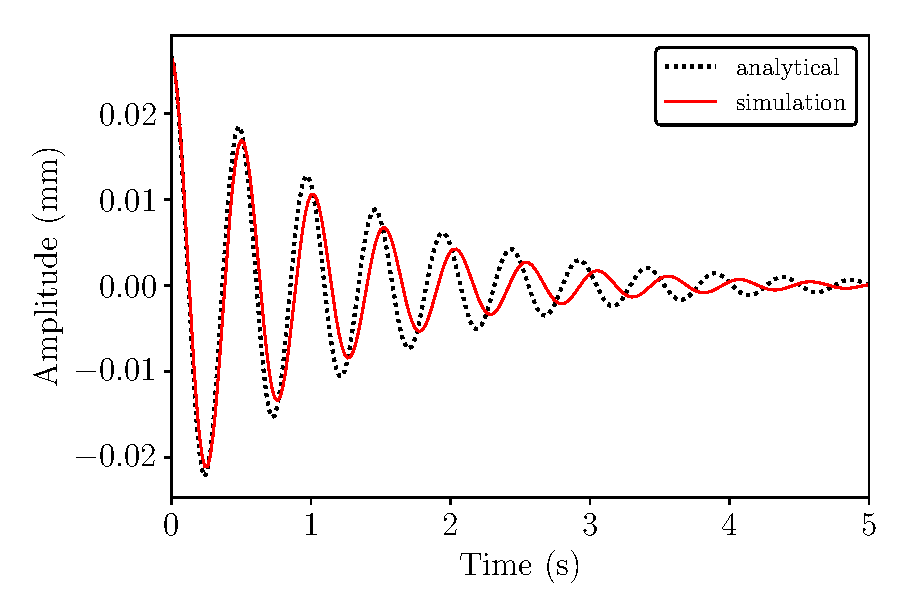
\includegraphics[height=5.3cm]{figures/wave_decay_4.eps} };
		\node (pic2) at (4,0)
		{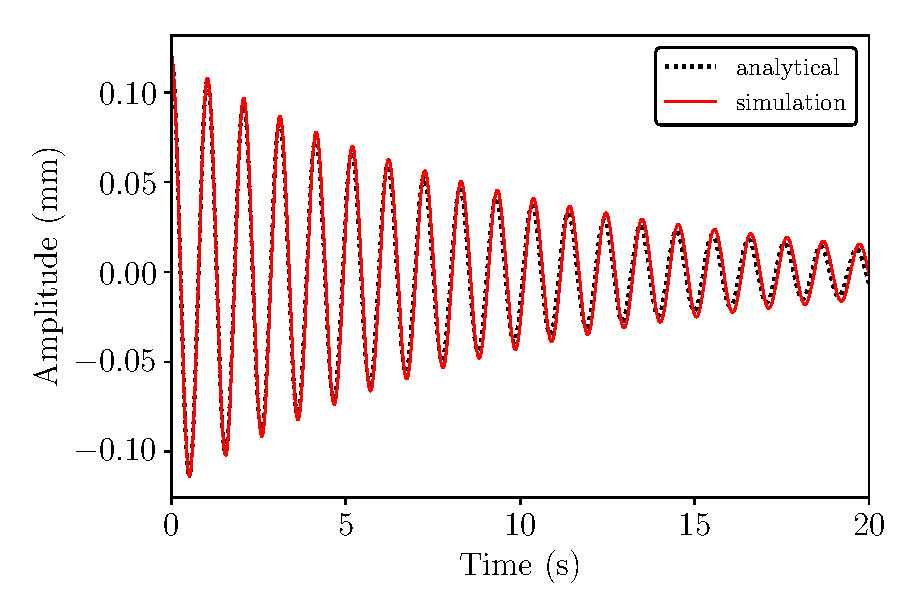
\includegraphics[height=5.3cm]{figures/wave_decay_18.eps} };
		\node [above of=pic1, xshift=-3.5cm, yshift=1.9cm] {$(a)$};
		\node [above of=pic2, xshift=-3.5cm, yshift=1.9cm] {$(b)$};
	\end{tikzpicture}
	\caption{The theoretical and simulated interfacial amplitude profiles for mode $(4,1)$ in a cell of length ($a$) $L_x=4$ cm and ($b$) $L_x=18$ cm and aspect ratio $L_x/L_y=3$. The initial amplitude given is $L_y/500$ m. The two-layer viscous damping equation succeeds in capturing the wave frequency and decay rate in the larger cell with a larger bulk flow regime.}
	\label{fig:wave_decay}
\end{figure}
%%%%%%%%%%%%%%

%%%%%%%%%%%%%%
\begin{figure}
	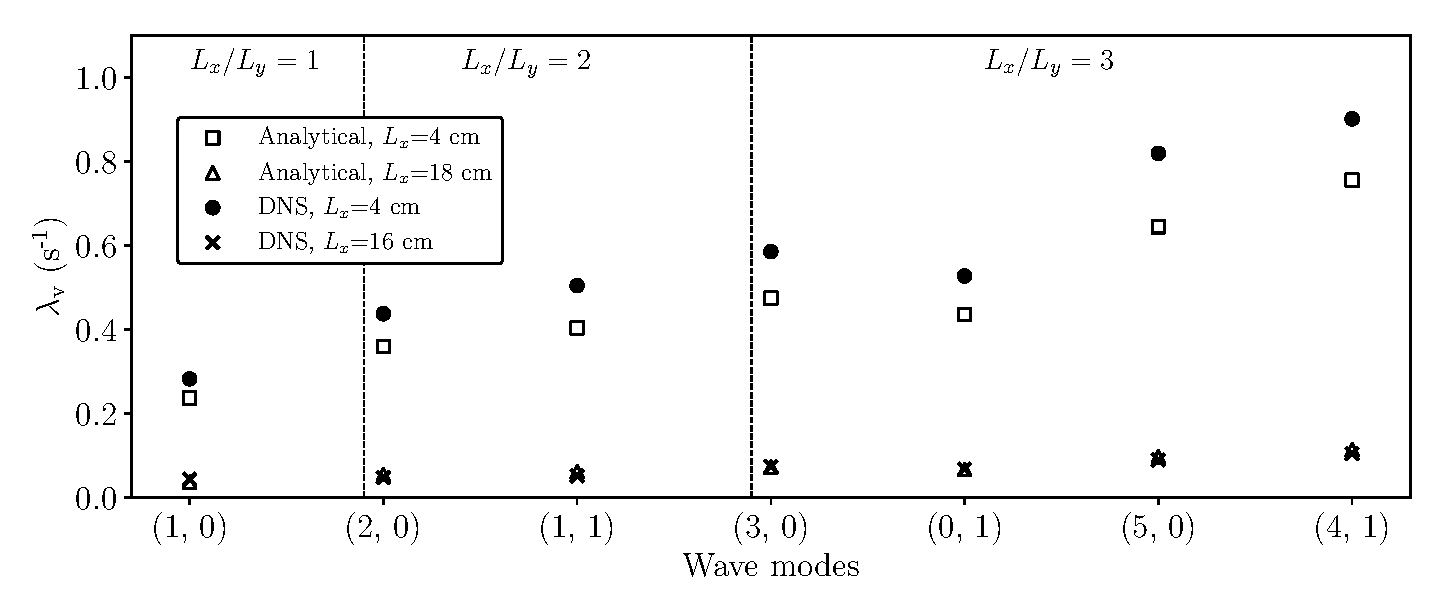
\includegraphics[width=0.9\linewidth]{figures/vDamp_coria_4cm_tot.eps}
	\caption{The comparison of the viscous damping rates for a two-layer cryolite-aluminum system in a rectangular geometry with the analytical viscous decay rates. The dimensions of the system are represented by length $L_x=4$ cm and layer heights $h_1, h_2= 0.5$ cm and length $L_x=18$ cm and layer heights $h_1, h_2= 2.25$ cm. The simulations were conducted in the most refined meshes obtained from grid dependency tests.}
	\label{fig:numeric_sim}
\end{figure}
%%%%%%%%%%%%%%


We have already shown that the viscous damping rate $\lambda$ agrees with the established linear damping rate in Eq. \,\eqref{eq:damp_1L_wall} derived by \citet{Keulegan1959} within its single-layer limit describing free-surface waves. However, interfacial waves are physically different because the leading-order viscous boundary layers form above and below the interface (the viscous boundary layer below a free surface is of higher order \citep{Joseph2006}), and Lamb's dissipation integral must be treated differently. However, the literature on two-layer interfacial wave damping is unfortunately rather limited. Therefore, we cross-validated the analytical results from Eqs.\,(\ref{eq:visc_damp_wall}\textendash\ref{eq:visc_damp_extra}) with DNS using ARCHER. For a two-layer (cryolite–aluminium) system similar to that of \citet{Politis2021}, barring the geometric dimensions with smaller lateral surface areas and equal layer heights, we initialized a standing interfacial wave profile of mode $(m,n)$ with a small amplitude of $L_z/500$ depending on the aspect ratio and let it decay over time. Three different cell aspect ratios (1, 2 and 3) with varying cell surface areas were simulated and compared with the theoretical values. The total surface areas were kept relatively small in order to reduce the computational cost. Due to the lack of sufficient models available to track the contact line motion of the interface, we were limited to an interfacial contact angle of $90^\circ$ and therefore, had to neglect the capillary effects on the lateral wall. The value of the interfacial tension was also set to zero. The comparisons done for a cell of smaller length $L_x=4$ cm and relatively larger length $L_x=18$ cm are presented in Fig.\,\ref{fig:numeric_sim}. A detailed explanation regarding the post processing of the decay rates is provided in Appendix\,\ref{appD}.
\\
\indent The solutions given by ARCHER in all cases follow the general trend of the theoretical values. Large deviations were observed for $L_x=4$ cm with an average deviation of 22\%, whereas the solutions converged for $L_x=18$ cm (average deviation of 10\%). Most experimental models like \citet{Pedcenko2009,Borisov2010} operate around this cell size or higher, therefore the agreement is quite promising. In smaller cell domains, the large deviations can be attributed to the viscous boundary layer ($\sqrt{\nu/\omega}$), which constitutes a significant portion (upwards of 10\%) of the layer height in smaller cells. In such cases, Potential theory is known to provide incorrect predictions \cite{Huang2025}.                 

\subsection{Comparison with \citet{LaRocca2002}}
\label{sec:visc_LaRocca}
\citet{LaRocca2002} conducted interfacial sloshing experiments in an enclosed square tank filled with two stably stratified liquid layers. These authors put one focus on dissipative effects and carried out direct decay rate measurements of different previously-excited interfacial wave modes. A theoretical model for viscous dissipation was also developed, without, however, providing an analytical expression for the damping rates. In Fig.\,\ref{fig:rocca_comparison} we compare Eq.\,\eqref{eq:visc_damp_sum} with La Rocca's results limited to cases where the authors provide both numerical and experimental data. Fig.\,\ref{fig:rocca_comparison}\hyperref[fig:rocca_comparison]{(a)} shows the non-dimensionalized viscous damping rate as a function of the non-dimensionalized kinematic viscosity for three different wave modes ($m,0$), $m=1,2,3$. Our linear damping theory slightly overshoots La Rocca's predictions but agrees even better with the three experimental measurements carried out at $\nu_1/(gL_y^3)^{1/2} = \SI{3.25e-5}{}$ and $\rho_1/\rho_2 = 0.85$.
%%%%%%%%%%%%%%
\begin{figure}
	\begin{tikzpicture}
		\node (pic1) at (-4,0) 
		{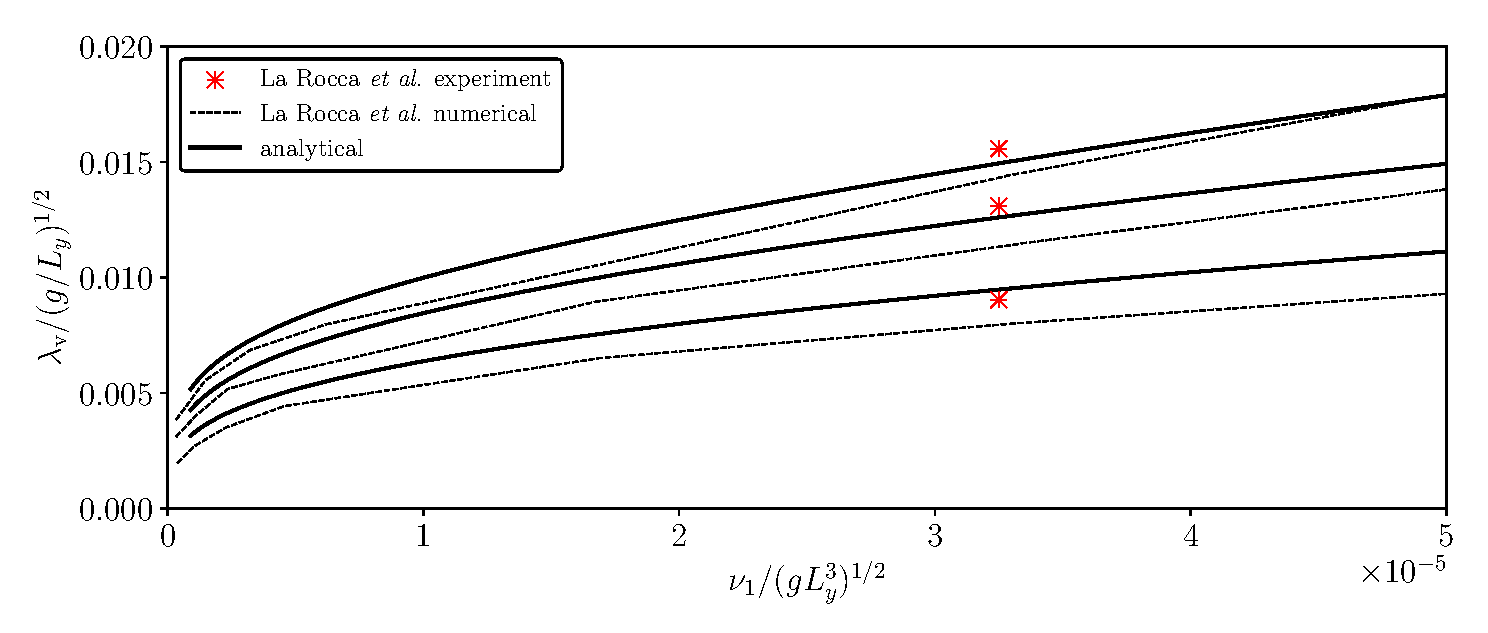
\includegraphics[height=5.5cm]{figures/rocca_viscosity.eps} };
		\node (pic2) at (4,0)
		{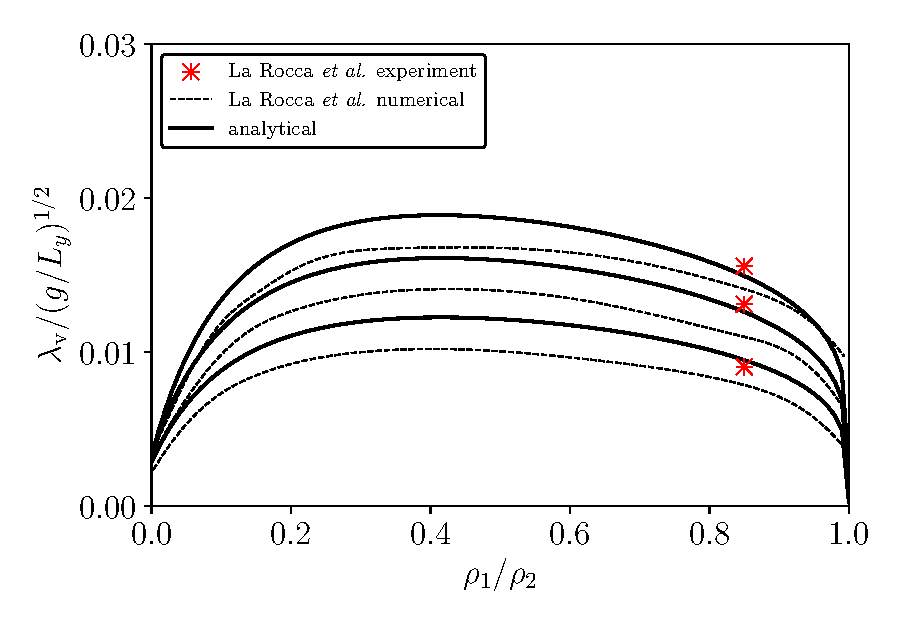
\includegraphics[height=5.5cm]{figures/rocca_density.eps} };
		\node [above of=pic1, xshift=-3.5cm, yshift=1.9cm] {$(a)$};
		\node [above of=pic2, xshift=-3.5cm, yshift=1.9cm] {$(b)$};
	\end{tikzpicture}
	\caption{($a$) Non-dimensionalized viscous damping rate as a function of the non-dimensionalized kinematic viscosity for three different unidirectional wave modes ($m,0$), $m=1,2,3$ at a constant density ratio of $\rho_1/\rho_2 = 0.85$. ($b$) non-dimensionalized damping rate as a function of the density ratio $\rho_1/\rho_2$ at a constant viscosity ratio ($\nu_1/\nu_2 \approx 36$) for the same wave modes. Additional measurement points are included for the first three modes $m=1,2,3$.}
	\label{fig:rocca_comparison}
\end{figure}
%%%%%%%%%%%%%%
The applicability of La Rocca's model, however is also limited, as is evident from Fig.\,\ref{fig:rocca_comparison}\hyperref[fig:rocca_comparison]{(b)}, showing the damping rate as a function of the density ratio $\rho_1/\rho_2$. This figure portrays the transition from free-surface to interfacial wave damping. In the limit of quasi free surfaces $\rho_1/\rho_2 \lesssim 0.1$ we find, as expected, very good agreement with our model. Their damping rate estimates tend to diverge at $\rho_1 = \rho_2$, which is physically incorrect as the wave's natural frequencies become infinitely small in the limit $\rho_1 \rightarrow \rho_2$ and, correspondingly, the waves must then attenuate infinitely slowly. Our solution exhibits the correct behavior and $\lambda$ vanishes at $\rho_1 = \rho_2$. Since we have  chosen exactly the same ansatz as \citet{Herreman2019}, who derived $\lambda$ for cylindrical geometries, and the decay rates have been successfully validated against measurements by \citet{Horstmann2019}, and had given good agreement with DNS simulations, we are convinced that our treatment of viscous damping is reliable given the applied approximations.

\subsection{Comparison with \citet{Politis2021}}
\label{sec:fractal}
We will show that the linear MPR growth rate and stability onset predictions by \citet{Politis2021} are fully contained in our model as a limiting case for $h_1 ,h_2 \ll L_x, L_y$, $\sigma_1 \ll \sigma_2$, $\gamma_{\ii{int}} = 0$ and constant damping coefficients. First, as a special case, we consider the growths of dissipationless MPR waves in inherently unstable cell configurations, for which \citet{Politis2021} derived a compact analytical expression. A cell is called inherently unstable whenever there exist two wave modes $(m,n)+(m',n')$, such that $(m+n) \land (m'+n')=\mathbb{N}_{\ii{odd}}$ and fulfilling $\delta \omega = 0$.
In shallow geometries, gravity waves are non-dispersive ($\omega = ck$, $\omega' = ck'$) and the frequency equality $\delta \omega = 0$ reduces to a wave number equality $k=k'$, imposing the following constraint on the lateral aspect ratio: 
\begin{align}
	k = \pi\sqrt{\frac{m^2}{L_x^2} + \frac{n^2}{L_y^2}} &= \pi\sqrt{\frac{m'^2}{L_x^2} + \frac{n'^2}{L_y^2}} = k' 
	\; \Longrightarrow \;  \frac{L_x^2}{L_y^2} = \frac{m'^2 - m^2}{n^2 - n'^2} = \frac{(m'-m)(m'+m)}{(n-n')(n+n')}.
\end{align}
This condition allows us to easily understand why the unstable aspect ratios form an absolutely discontinuous dense set of points. 
For a simple explanation, let us first consider the wave mode function $\Theta$ [Eq.\,\eqref{eq:form_function}], which can only be non-zero if both wave mode pairs $(m,m')$ and $(n,n')$ are of opposite parity. Wave pairs whose wave modes $(m,m')$ or $(n,n')$  are both even or odd can therefore never be destabilized. From number theory it is known that all sums and differences
of numbers with opposite parity yield odd numbers $m \pm m' = {\rm odd}$ and $n \pm n' = {\rm odd}$. Likewise, products of odd numbers are again always odd, which is why we can assign
\begin{align}
	\frac{(m'-m)(m'+m)}{(n-n')(n+n')} = \frac{M}{N}, \label{eq:fractal}
\end{align} 
where $M$ and $N$ are any two odd numbers. The fractality of the unstable aspect ratios can be described by $L_x/L_y = \sqrt{M/N}$ \cite{Politis2021}. From Eq.\,\eqref{eq:fractal} we can deduce the most unstable wave pair for all cells fulfilling $L_x/L_y = \sqrt{M/N}$ in the inviscid limit: 
\begin{equation}
	m = \frac{M-1}{2}, \quad m' = \frac{M + 1}{2}, \qquad
	n = \frac{N +1}{2}, \quad n' = \frac{N - 1}{2}	.
	\label{eq:mn_odd}
\end{equation}
By inserting the most unstable wave numbers [Eq.\,\eqref{eq:mn_odd}] into the growth rate solution in Eq.\,\eqref{eq:main_gr} and applying all the mentioned limits we obtain an expression for $\alpha_{\rm MPR}$ as a function of the fractal numbers
\begin{equation}
	\alpha_{\rm MPR} = \pm \, \beta_{\rm S} \: \frac{c}{\sqrt{L_xL_y}} \frac{8}{\pi^3}
	\sqrt{\frac{\delta_{M-1}\delta_{N-1}}
		{(M + N)(MN+1)\sqrt{MN}}}.
	\label{eq:priede_dimension}
\end{equation}
%%%%%%%%%%%%%%%
The above Eq.\,\eqref{eq:priede_dimension} (see Eq.\,\eqref{eq:delta_func} for $\delta_{M-1}, \delta_{N-1}$) is the dimensional form of the growth rate solution [Eq.\,(3.28)] of \citet{Politis2021}, which verifies the equivalence of both models. It remains to validate our predictions of stability onsets, which \citet{Politis2021} have presented in the form of critical Sele parameters $\beta_{\ii{crit}}$ and studied their dependence on the aspect ratio. For this purpose, the authors also modeled damping by introducing a phenomenological friction coefficient $\gamma$. However, the resulting eigenvalue problem was only solved numerically using the Galerkin method, and for this reason we compare the onset solutions graphically in the following. Although we have derived an explicit analytical solution for $\beta_{\rm crit}$, Eq.\,\eqref{eq:beta_crit-onset}, it is not evident \textit{a priori} which mode pair is most unstable and thus defines $\beta_{\rm crit}$. Considering damping and operating beyond the shallow-water approximation, the most unstable mode pair cannot be determined analytically. Our simple strategy for solving this problem is to calculate $\beta_{\rm crit}$ for all possible combinations of wave pairs and then to assign $\beta_{\rm crit}$ to the particular wave pair that yields the lowest onset value. The smallest possible critical Sele parameter defines the global instability onset. However, this iterative method is not a major limitation for our model because large-scale wave modes are always most unstable in practice, such that only wave numbers up to about $m,n \lesssim 10$ must be examined. This is because damping increases markedly with increasing wave numbers and also because small-scale wave motions are gradually suppressed by interfacial tension ($\beta_{\gamma_{\ii{int}}}$ in Eq.\,\eqref{eq:beta_crit-onset} diminishes with increasing $k$).
%%%%%%%%%%%%%
\begin{figure}
	\centering
	\begin{tikzpicture}
		\node (pic1) at (0,0)  {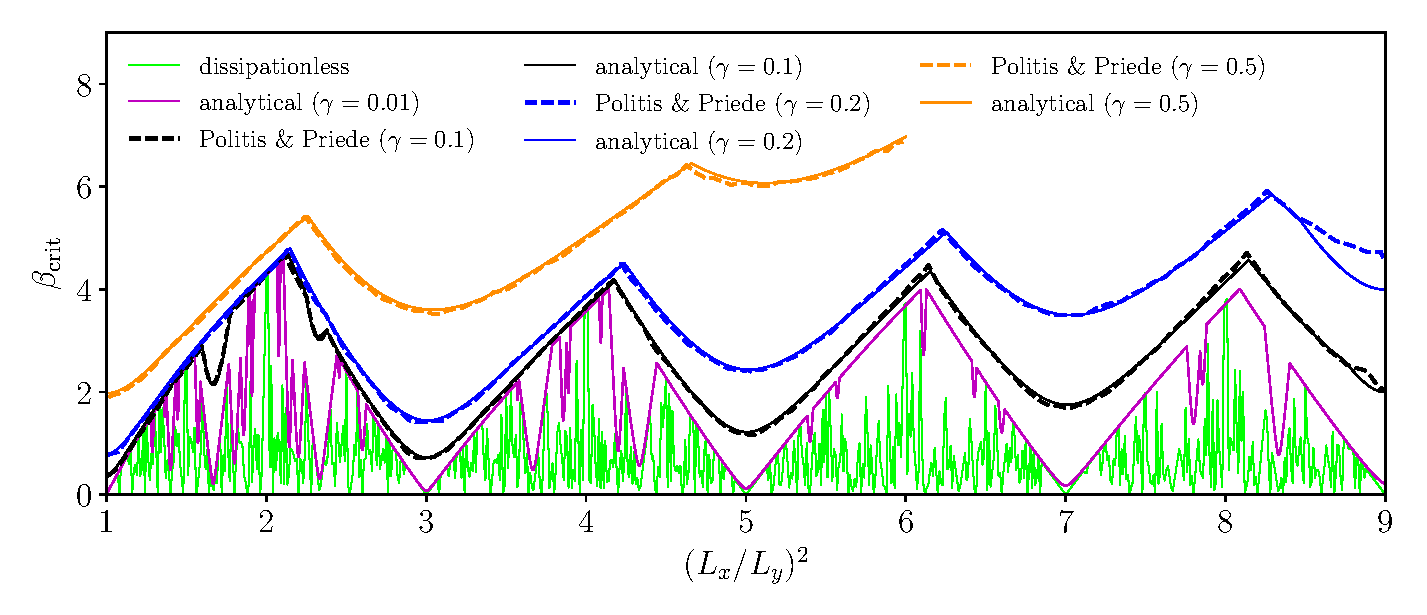
\includegraphics[width=0.9\linewidth]{figures/priede_fractal.eps} };
		\node (pic2) [below of=pic1, yshift=-5.8cm]
		{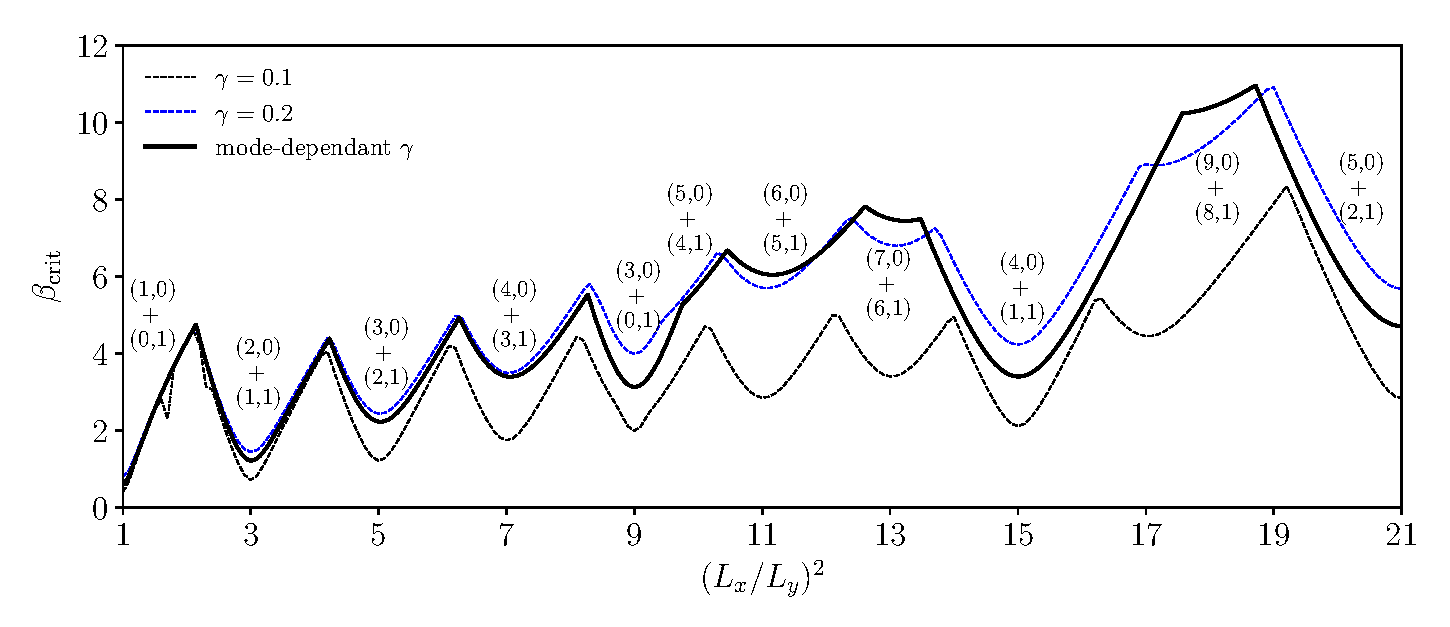
\includegraphics[width=0.9\linewidth]{figures/priede_ph_fractal.eps} };
		\node (a) at (-7.1,3.6) {$(a)$};
		\node (b) [below of=a, yshift=-5.9cm] {$(b)$};
	\end{tikzpicture}
	\caption{ Critical Sele parameters $\beta_{\ii{crit}}$ from \citet{Politis2021} and our analytical prediction [Eq.\,\eqref{eq:beta_crit-onset}] as a function of the aspect ratio squared $(L_x/L_y)^2$, with and without considering the effects of damping here modeled by (a) arbitrary constant damping coefficients $\gamma$. The non-dimensional coefficients $\gamma$ were re-dimensionalized as $\lambda=0.5\gamma \, c/L_x$ and $\lambda'=0.5\gamma\, c/L_y$. The red curves show the approximate solution [Eq.\,\eqref{eq:beta_approx}] for $\gamma=0.2$ around $L_x/L_y = \sqrt{3}$ and $L_x/L_y = \sqrt{5}$. In (b) the instability onsets are plotted for variable friction coefficients calculated from damping rates in Eq.\,\eqref{eq:visc_damp_sum} for aspect ratios squared extending till 21.}
	\label{fig:priede_fractal}
\end{figure}
%%%%%%%%%%%%%

Fig.\,\ref{fig:priede_fractal}\hyperref[fig:priede_fractal]{(a)} shows iteratively calculated onset values $\beta_{\rm crit}$ as a function of the squared lateral aspect ratio $(L_x/L_y)^2$ compared with numerical solutions by \citet{Politis2021} for different friction coefficients $\gamma$. All geometrical parameters and material properties of the considered cell are given in Table\,\ref{tab:table_properties}. We find a quasi-perfect agreement between both models for any given friction coefficient. The pattern of the green fractal curve ($\gamma = 0$) is determined solely by the chosen resolution. All other curves can be unambiguously determined; the non-differentiable inflection points indicate the transitions between different most unstable wave pairs. Fig.\,\ref{fig:priede_fractal}\hyperref[fig:priede_fractal]{(b)} provides the analytical prediction from Eq.\,\eqref{eq:beta_crit-onset} taking into account viscous damping from Eq.\,\eqref{eq:visc_damp_sum}, highlighting all the unstable wave modes between the inflection points. Extending the graph until the aspect ratio square of 21 shows us why most industrial ARCs operate at $(L_x/L_y)^2=17$\textendash$18$, due to the presence of a larger stability buffer \cite{Zhang2011}. Using Fig.\,\ref{fig:priede_fractal}\hyperref[fig:priede_fractal]{(b)}, it is possible to explain the small deviation emerging between our respective theories at $\gamma = 0.2$ for $(L_x/L_y)^2 > 8.45$ in Fig.\,\ref{fig:priede_fractal}\hyperref[fig:priede_fractal]{(a)}. The curve from \citet{Politis2021} shows here $\beta_{\ii{crit}}$ for the mode pair $(5,0)+(4,1)$. However, our solution predicts that the pair $(3,0)+(0,1)$ becomes unstable first, and accordingly our calculated curve is slightly lower. Apart from this point, however, the most unstable wave pair is always correctly predicted by the wave number tuples [Eq.\,\ref{eq:mn_odd}]. For these cases, a simple approximate solution for $\beta_{\rm crit}$ can be derived from our theory that is valid in the vicinity of the most unstable aspect ratios ($L_x^2/L_y^2 = 1,3,5,\dots$). Given these aspect ratios, we can set $N=1$, because $L_x^2/L_y^2 = M/1$ with $M=1,3,5,\dots$, and, by introducing Eq.\,\eqref{eq:mn_odd} into \eqref{eq:beta_crit_shallow}, ignoring the term $i\delta\omega\delta\lambda$ and re-dimensionalising  $\lambda=0.5\gamma \, c/L_x$ and $\lambda'=0.5\gamma\, c/L_y$, $\beta_{\rm crit}$ can be deduced as a function of only $L_x/L_y$ and $M$:
\begin{equation}
	\beta_{\ii{crit}}= \frac{\pi^4 \sqrt[4]{M}
		(M+1) }{16\sqrt{\delta_{M-1}}}\sqrt{
		\frac{\gamma^2}{\pi^2} + \frac{L_y}{2L_x} (M^2+1) + \frac{L_x}{L_y} - \sqrt{
			\frac{(M^2 -1)^2}{4}\,\frac{L_y^2}{L_x^2} + (M+1)^2}}. \label{eq:beta_approx}
\end{equation}
%%%%%%%%%%%%%%%%
In this approximation, the numbers $M$ must be taken as constants and the aspect ratio $L_x/L_y$ as a variable. For $\gamma=0.2$, we show Eq.\,\eqref{eq:beta_approx} by the red curves for $M=3$ and $M=5$ in Fig.\,\ref{fig:priede_fractal}\hyperref[fig:priede_fractal]{(a)}. The approximate solution is very accurate, but deviations become evident near the wave mode transition peaks so that the most stable aspect ratios cannot be determined analytically from Eq.\,\eqref{eq:beta_approx}. Onset values for the most unstable aspect ratios $L_x/L_y = 1,3,5,\dots$, however, can readily be derived from Eq.\,\eqref{eq:beta_approx} by setting $L_x/L_y = \sqrt{M}$ yielding the exact solution 
\begin{equation}
	\beta_{\ii{crit}}= \frac{\pi^3 \sqrt[4]{M}
		(M+1) }{16\sqrt{\delta_{M-1}}}\gamma. \label{eq:beta_min}
\end{equation}
The physical relevance of the fractal distribution of critical aspect ratios, which is enveloped by the dissipative curves, has already been discussed in detail by \citet{Politis2021}. We make here a final note that the most unstable wave pairs (smallest $\beta_{\rm crit}$) are not always the wave pairs with the highest growth rate. Therefore, other mode pairs than these predicted at $\beta_{\rm S} = \beta_{\rm crit}$ can develop at higher $\beta_{\rm S} > \beta_{\rm crit}$, which is why the exact pattern of MPR waves is difficult to predict even in the linear regime.
At some certain point $\beta_{\rm S} > \beta_{\ii{crit}}$, it is always the primary rotating mode pair $(1,0)+(0,1)$ that yields the highest growth rate in all possible cell configurations, as already noted by \citet{Munger2008}. But in these high $\beta_{\rm S}$ regimes, linear MPR models are often no longer applicable. 


\subsection{Comparison with measured stability onsets by \citet{Borisov2010}}
\label{sec:Borisov}

As \citet{Politis2021} have adopted constant damping parameters, it remains to compare our onset solution [Eq.\,\eqref{eq:beta_crit-onset}] in conjunction with wave mode-dependent damping rates (\ref{eq:visc_damp_sum}), which constitute the major amelioration of our model. For this, the overlooked one-of-a-kind experiment by \citet{Borisov2010} is the perfect (and only) option. The authors are the only ones to have ever succeeded in destabilizing MPR waves in two-layer experimental cells that can reproduce the complete MPR magnetohydrodynamics without any noteworthy trade-off. In their set-up, two transparent liquids were stratified (nitric acid ($\rm{HNO}_{\rm{3(aq)}}$ at the bottom and $\rm{HNO}_{3}$ + ${\rm C}_5\rm{H}_{12}\rm{O}$ at the top), both of which had small but sufficiently contrasting electrical conductivities ($\sigma_1 = 0.67\,{\rm S}\,{\rm m}^{-1}$ and $\sigma_2 = 47.5\,{\rm S}\,{\rm m}^{-1}$). Due to the comparatively small difference in the density of the two liquids, small cell currents  $I \sim 2$ \textendash \ $4\,{\rm A}$, in combination with a strong external magnetic field  $B_z = 0.25\,{\rm T}$, were sufficient to attain large enough Sele parameters $\beta_{\rm S} \sim 2$ to destabilize MPR waves. In order to change the electrical boundary conditions at the bottom electrode, the authors employed a removable insert made of porous material that was impregnated with an aqueous solution of nitric acid. This allowed both sets of idealized boundary conditions to be realized in the experiment, i.e. that the lower liquid be either a much better or much worse electrical conductor than the bottom electrode. Unfortunately, the authors have only published measurements without the insert, for which the ground electrode can be regarded as a perfect electrical conductor. This configuration is not accounted for by our model, but simply by changing the Neumann boundary condition [Eq.\,\eqref{eq:bc4}] to the Dirichlet boundary condition $\varphi_2 = 0|_{z=-h_2}$, we can easily adapt our solution. The stability onset has the same form as before:
%%%%%%%%%%%%%%%%
\begin{equation}
	\beta_{\ii{crit}} = \frac{L_x^2 L_y^2}{h_1h_2 \Theta}
	\sqrt{ \frac{\overbar\lambda^2 - \bigl[ \ii i{\delta \omega} -\delta\lambda \bigr]^2} {(\overbar\omega^2 - {\delta\omega}^2) \mathcal{T}_c\mathcal{T}'_c} } ,
	\label{eq:beta_crit_cond}
\end{equation}
%%%%%%%%%%%%%%%%
where,
\fontsize{11pt}{11pt}
\begin{align*}
	\mathcal{T}_c &= \dfrac{\Lambda}{k(k^2 - k'^2)}
	\Biggl[ 
	\dfrac{-k'}{\text{tanh}[kh_1]} 
	+ \dfrac{k'\:\text{sech}[k'h_1]}{\text{sinh}[kh_1]}
	+ \dfrac{k}{\text{coth}[k'h_1]}
	+ \dfrac{-k'}{\text{tanh}[kh_2]} 
	+ \dfrac{k'\:\text{sech}[k'h_2]}{\text{sinh}[kh_2]}
	+ \dfrac{k}{\text{coth}[k'h_2]}
	\Biggr] ,
	\\[5pt]
	\mathcal{T}'_c &= \dfrac{\Lambda'}{k'({k'}^2-k^2)}
	\Biggl[ 
	\dfrac{-k}{\text{tanh}[k'h_1]} 
	+ \dfrac{k\: \text{sech}[kh_1]}{\text{sinh}[k'h_1]}
	+ \dfrac{k'}{\text{coth}[kh_1]}
	+\dfrac{-k}{\text{tanh}[k'h_2]} 
	+ \dfrac{k\: \text{sech}[kh_2]}{\text{sinh}[k'h_2]}
	+ \dfrac{k'}{\text{coth}[kh_2]}
	\Biggr] ,
\end{align*}
\normalsize
and the new conductivity jump parameter is
\[
\Lambda = \dfrac{\sigma^{-1}_1-\sigma^{-1}_2}{\sigma^{-1}_1\ii{tanh}[kh_1] + \sigma^{-1}_2\ii{tanh}[k h_2]}	.
\]
%%%%%%%%%%%%%%%%
\begin{figure}
	\centering
	\begin{tikzpicture}
		\node (pic1) at (0,0)  {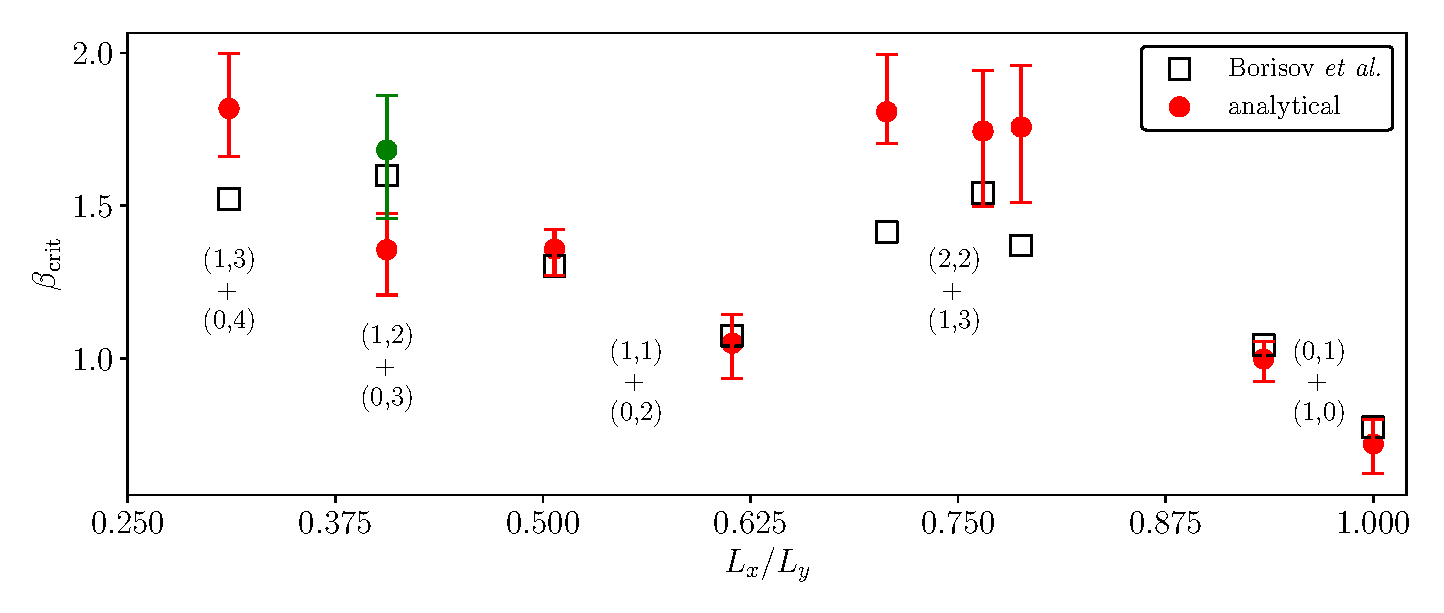
\includegraphics[width=0.9\linewidth]{figures/theory_vs_Borisov_calculated.eps} };  
		\node (pic2) [below of=pic1, yshift=-6cm] {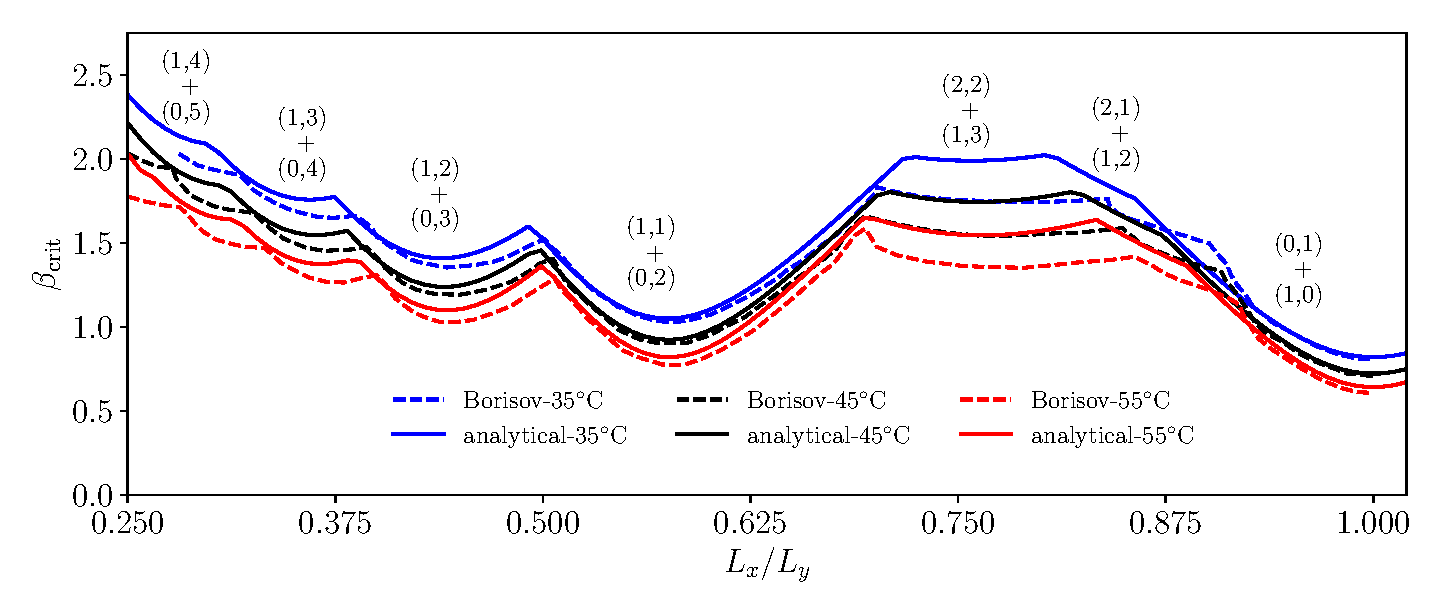
\includegraphics[width=0.9\linewidth]{figures/theory_vs_Borisov_lines.eps} }; 
		\node [below of=pic2, yshift=-6cm] {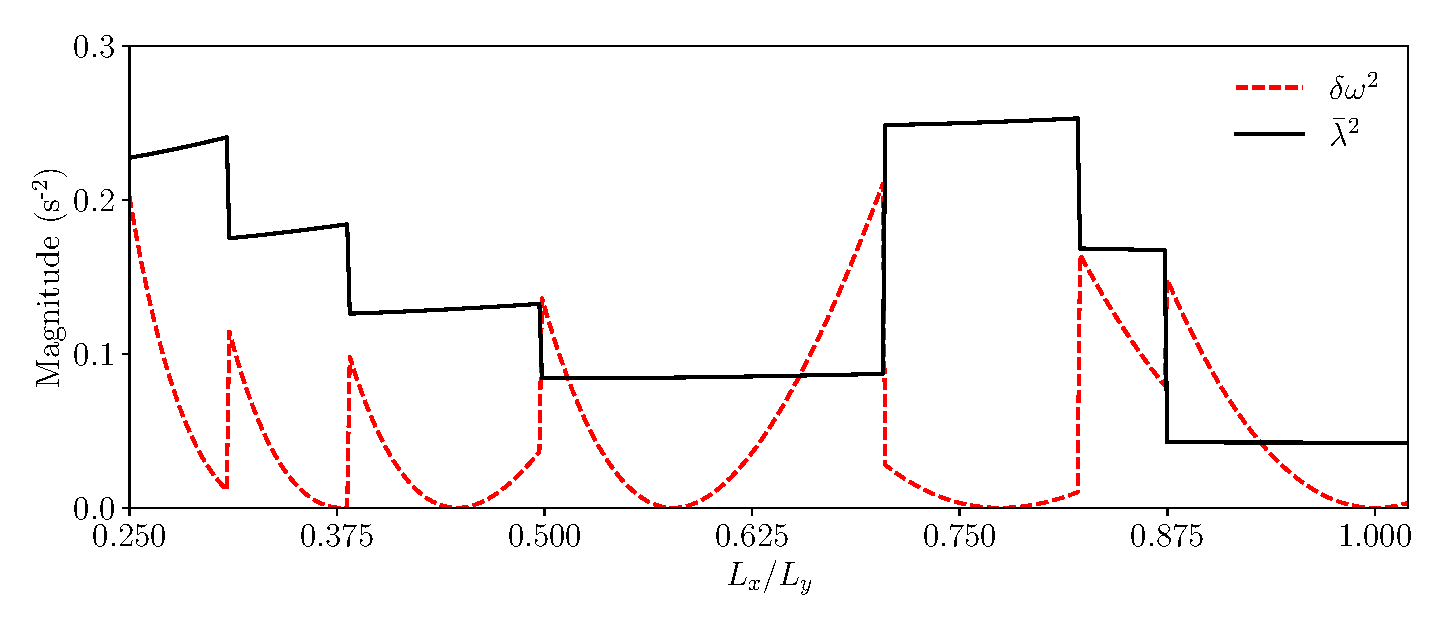
\includegraphics[width=0.9\linewidth]{figures/Borisov-total-damping.eps} };
		\node (a) at (-7.1,3.4) {$(a)$};
		\node (b) [below of=a, yshift=-6cm] {$(b)$};
		\node [below of=b, yshift=-5.9cm] {$(c)$};
	\end{tikzpicture}
	\caption{(a) Comparison with the experimentally observed stability onsets at nine different cell geometries. The error bars cover a temperature range of $35^{\circ}$C to $55^{\circ}$C. (b) shows the analytical stability onset comparisons along with the critical wave modes observed at different cell aspect ratios. (c) is the distribution of parameters $\delta\omega^2$ and $\overbar\lambda^2$ which play a key role in determining the critical wave mode and therefore, the critical onset value.}
	\label{fig:borisov_comparison}
\end{figure}
%%%%%%%%%%%%%%%%%

Here, \citet{Borisov2010} measured the critical onsets using a different dimensionless parameter $W = I_0 B_z /[(\rho_2 - \rho_1)gL_x L_y]$ that can easily be rewritten as $\beta_{\rm S}$ through $\beta_{\rm S} = W\:L_xL_yh_1^{-1}h_2^{-1}$. The measured critical Sele parameters are shown together with the most unstable wave pairs $(m,n) + (m',n')$ in 9 different cells of different aspect ratios $L_x/L_y$ in Fig.\,\ref{fig:borisov_comparison}\hyperref[fig:borisov_comparison]{(a)}. For a better understanding, Fig.\,\ref{fig:borisov_comparison}\hyperref[fig:borisov_comparison]{(b)} further shows our continuous solution [Eq.\,\eqref{eq:beta_crit_cond}] compared with the stability prediction from a linear non-shallow MPR theory developed by \citet{Borisov2008}, who used the Galerkin method to formulate a Cauchy problem that was solved numerically. Fig.\,\ref{fig:borisov_comparison}\hyperref[fig:borisov_comparison]{(c)} supplements Fig.\,\ref{fig:borisov_comparison}\hyperref[fig:borisov_comparison]{(b)} and shows the proportion of the two key parameters $\bar{\lambda}^2$ and $\delta \omega^2$ in Eq.\,\eqref{eq:beta_crit-onset}, allowing the reader to determine whether a given onset value $\beta_{\rm crit}$ is influenced more by total damping or frequency mismatching. During their experiments, \citet{Borisov2010} had to contend with the difficulty that the cell was subject to strong temperature fluctuations due to the high Ohmic losses (Joule heating) occurring in both poorly conducting liquids. The authors measured  temperatures between $35^{\circ}-55^{\circ}$C, which we incorporated in Fig.\,\ref{fig:borisov_comparison}\hyperref[fig:borisov_comparison]{(a)} using error bars. At all examined aspect ratios the reported wave pairs coincide with the most unstable pairs predicted by our model. Quantitatively, we also find fair agreement, but there are some considerable deviations, especially for the mode pair $(2,2) + (1,3)$. The measurement point that corresponds to $(1,2) + (0,3)$ lies very close to the jump point between the most unstable pairs $(1,2) + (0,3)$ and $(1,3) + (0,4)$, see Fig.\,\ref{fig:borisov_comparison}\hyperref[fig:borisov_comparison]{(c)}. If we pick the neighbouring pair $(1,3) + (0,4)$ (green measuring point) here, although our model still predicts $(1,2) + (0,3)$ to be most unstable, we also find good agreement within the scope of measurement accuracies. In general, it can be observed that those measurements with the highest deviations also differ the most from Borisov's theory. The direct comparison of both theories reveals that our model always yields larger $\beta_{\rm crit}$. Due to difficulties arising from translation, the reason for this discrepancy is quite difficult to identify, but we noticed that \citet{Borisov2010} have entirely neglected sidewall damping. This is a misconception, we have estimated from our damping rates in Eqs.\,\eqref{eq:visc_damp_wall}, \eqref{eq:visc_damp_interface} and \eqref{eq:visc_damp_extra} that sidewall damping in this non-shallow two-layer cell accounts for more than a third of the total damping. Despite this stark difference, both theories concur remarkably well, so there must be other differences in the modeling that we cannot elaborate on further. Due to the completeness of our theory and the compatibility with many previous MPR models, we are convinced that the larger $\beta_{\rm crit}$ parameters predicted by our model are physically reasonable. We hope to dispel any remaining doubts in the future with our own MPR experiment \citep{Hegde2025}, which permits precise and direct measurement of the growth rate $\alpha_{\rm MPR}$ and the damping rate $\lambda$ in addition to $\beta_{\rm crit}$.


\section{Concluding remarks}
\label{sec:discuss}

Our explicit perturbation formulation of the linear MPR instability resulting from two superimposed transverse standing wave modes extends existing MPR models so that we can accurately describe small-scale MPR models. This is done so by overcoming the shallow-water approximation and taking capillary wave regimes into account. The most important refinement, however, is that we consider dissipation not only in terms of purely phenomenological damping parameters, but explicitly calculate the wave mode-dependent viscous damping rates. Because the resultant dissipation can differ considerably from wave mode to wave mode, see Fig.\,\ref{fig:borisov_comparison}\hyperref[fig:borisov_comparison]{(c)}, this makes a sizable difference to the global stability.
\\
\indent We have gone to great lengths to keep all analytical solutions explicit and as tangible as possible so that these can be implemented with minimal efforts and without a wealth of prior knowledge. The main result of our study is provided by Eq.\,\eqref{eq:main_gr}, which predicts MPR growth rates $\alpha_{\rm MPR}$ for any given pair of standing wave modes. In a simple way, the global stability behavior is contained in this single equation: whenever the square root in Eq.\,\eqref{eq:main_gr} yields a complex number with zero real part, the cell remains stable and only the natural frequencies of the waves are shifted by MHD coupling effects. If the real part of the square root turns nonzero but the real part of $\alpha_{\rm MPR}$ is negative, excited waves still attenuate, but more slowly than they would without MHD coupling, and both waves oscillate at the same frequency. Once the real part of $\alpha_{\rm MPR}$ finally attains a positive value, the cell becomes MPR unstable and an exponentially growing rotating wave motion builds up at the interface. The growth rate $\alpha_{\rm MPR}$ incorporates the individual damping rates $\lambda$ and $\lambda'$ of the two coupled standing waves, which we have calculated separately. To account for viscous damping, we have calculated the leading-order Stokes boundary layers forming at all container walls as well as above and below the interface, and evaluated Lamb's dissipation integral [Eq.\,\eqref{eq:dissip}]. The total damping rate $\lambda$ [Eq.\,\eqref{eq:visc_damp_sum}] is composed of a wall damping term [Eq.\,\eqref{eq:visc_damp_wall}], an interfacial damping term [Eq.\,\eqref{eq:visc_damp_interface}] and a term resulting from the irrotational flow [Eq.\,\eqref{eq:visc_damp_extra}]. Regardless of the MPR instability, these damping rates can be used for other problems such as for two-liquid sloshing experiments, and can further serve as an easy benchmark for direct numerical solvers, e.g. to verify whether the viscous boundary layers have been resolved sufficiently, as demonstrated in Sec.\,\ref{sec:visc_simulation}. Due to the complex dependencies of the damping rates on the wave modes, our model cannot in general predict which wave pair will be destabilized first, as is possible in the limiting case of shallow layers and constant damping, see Sec.\,\ref{sec:fractal}. Therefore, it is necessary to calculate the most unstable wave mode pair, which defines the critical stability parameter $\beta_{\rm crit}$ in Eq.\,\eqref{eq:beta_crit-onset}, iteratively. To simplify the calculations for the reader, we have gathered all essential equations in Appendix\,\ref{appC} and added some explanations for easy implementation.
\\
\indent This stability theory is intended to calibrate our recent single-layer MPR experiment \cite{Hegde2025} in such a way that it can properly reflect the magnetohydrodynamics of (idealized) aluminum reduction cells. Then, for the first time, we will be able to measure and benchmark MPR growths rates of individual wave pairs. Moreover, our theory is well-positioned for augmenting the cell current (or external magnetic field) with alternating components, with a view to studying active MPR suppression techniques that have recently proved promising \cite{Mohammad2022}. In \citet{Horstmann2025} it was shown that the alternating current MPR suppression rests in a special form of parametric anti-resonance. However, the analysis relied on a highly idealized pendulum model with only two degrees of freedom. The ideal AC frequencies for a minimally-invasive MPR suppression predicted in \cite{Horstmann2025} still need to be confirmed by continuous MPR theories.











% Specify following sections are appendices. Use \appendix* if there
% only one appendix.
\appendix
\section{Formulation of the Fredholm alternative} \label{appA}

The balance Eqs.\,\eqref{eq:gov_momentum} and \eqref{eq:gov_cont} considering only leading order terms, for a given wave mode $(m,n)$ are
%%%%%%%%%%%%%%%%%%%%
\begin{subequations}
	\begin{equation}
		\rho_i(\ii i\omega - \lambda)\widehat{\h u_i} + \bm\nabla\widehat p_i = 0 ,
		\label{eq:lead_balance_1}
	\end{equation}
	\begin{equation}
		\bm\nabla \cdot \widehat{u_i} = 0 ,
		\label{eq:lead_balance_2}
	\end{equation}
	\begin{equation}
		\widehat{\h j}_i  = -\sigma_i \bm\nabla\widehat\varphi_i , 
		\qquad \bm \nabla \cdot \widehat{\h j}_i=0 .
		\label{eq:static_ohmslaw}
	\end{equation}
\end{subequations}
The complete expression when we input the ansatz [Eq.\,\eqref{eq:perturb_method_ansatz}] in the momentum Eq.\,\eqref{eq:gov_momentum} is given as
\begin{align}
	\nn
		&C\bigl(\ii i\overbar\omega + \alpha - \overbar\lambda \bigr)\rho \widehat{\h{u}} 
		+ 
		C'\bigl(\ii i\overbar\omega + \alpha - \overbar\lambda \bigr)\rho \widehat{\h{u}}'
		+ (\ii i\overbar\omega + \alpha - \overbar\lambda)\widetilde{\h{u}} + \bm{\nabla}\widetilde{p} 
		+ (\ii i\overbar\omega + \alpha - \overbar\lambda)\widetilde{\h{u}}' + \bm{\nabla}\widetilde{p}'
		\\
		= \;
		&C \Bigl( \:\widehat{\h{j}} \times B_z\bm{e}_z\Bigr) 
		+ 
		C' \Bigl( \:\widehat{\h{j}}' \times B_z\bm{e}_z\Bigr)
	\label{eq:pre_fredholm_step}
\end{align}
On expanding $\overbar\omega$ and $\overbar\lambda$ on the LHS of Eq.\,\eqref{eq:pre_fredholm_step}, we get the following:
\begin{align}
	\nn \Longrightarrow
		C&\bigl(\ii i\omega - \ii i\delta\omega + \alpha - \lambda + \delta\lambda \bigr)\rho \widehat{\h{u}} 
		+ 
		C'\bigl(\ii i\omega - \ii i\delta\omega + \alpha - \lambda + \delta\lambda \bigr)\rho \widehat{\h{u}}'
		\\
		+ 
		&(\ii i\omega - \ii i\delta\omega + \alpha - \lambda + \delta\lambda)\widetilde{\h{u}} + \bm{\nabla}\widetilde{p} 
		+ 
		(\ii i\omega - \ii i\delta\omega + \alpha - \lambda + \delta\lambda)\widetilde{\h{u}}' + \bm{\nabla}\widetilde{p}',
	\label{eq:pre_fredholm_step2}
\end{align}
%%%%%%%%%%%%
We now make certain leading order approximations  $\omega\widetilde{\h u}_i \gg \delta\omega \widetilde{\h u_i}$ and $\lambda\widetilde{\h u}_i \gg \delta\lambda \widetilde{\h u_i}$, to simplify Eq.\,\eqref{eq:pre_fredholm_step2} as
\begin{align}
	\nn
		&C\bigl(-[\ii{i} \delta\omega - \delta\lambda] + \alpha \bigr)\rho \widehat{\h{u}} 
		+ 
		C'\bigl([\ii{i} \delta\omega  - \delta\lambda] + \alpha\bigr)\rho \widehat{\h{u}}'
		 + 
		(\ii{i}\omega - \lambda)\widetilde{\h{u}} + \bm{\nabla}\widetilde{p} 
		+ 
		(\ii{i}\omega' - \lambda')\widetilde{\h{u}}' + \bm{\nabla}\widetilde{p}'
		\\ = \;
		&C \Bigl( \:\widehat{\h{j}} \times B_z\bm{e}_z\Bigr) 
		+ 
		C' \Bigl( \:\widehat{\h{j}}' \times B_z\bm{e}_z\Bigr),
\end{align}
\begin{align}
	\nn
	&\Longrightarrow
		(\ii{i}\omega - \lambda)\rho\widetilde{\h{u}} + 
		\bm{\nabla}\widetilde{p} 
		+ 
		(\ii{i}\omega' - \lambda')\rho\widetilde{\h{u}}' + 
		\bm{\nabla}\widetilde{p}'
		\\
	&=
		C \Bigl( \: \widehat{\h{j}} \times B_z\bm{e}_z
		+
		\Bigl( [\ii{i} \delta\omega - \delta\lambda] - \alpha \Bigr)\rho \widehat{\h{u}}\Bigr) 
		+ 
		C' \Bigl( \:\widehat{\h{j}}' \times B_z\bm{e}_z
		+
		\Bigl( -[\ii{i} \delta\omega - \delta\lambda] - \alpha \Bigr)\rho \widehat{\h{u}}'
		\Bigr).
	\label{eq:wavepack_first}
\end{align}
Applying the Fredholm alternative to the equations over the two fluid regions as follows:
\begin{equation}
	\Sigma_{i=1,2} \int_{V_i} \left[ \widehat{\h u}^*_i \cdot [\ii{Eq.\,\eqref{eq:wavepack_first}}] + \widehat p^*_i(\bm\nabla \cdot \widetilde{\h u}_i) \right] \ii dV,
\end{equation}
we can write the inner product (for quantities pertaining to wave mode $(m,n)$) as
%%%%%%%%%%%%
\begin{equation}
	\begin{array}{rl}
		&
		\sum_{i=1,2} \int_{V_i} \Bigl[ C \widehat{\h u}_i^{*} \cdot 
		\Bigl( 
		[\ii{i} \omega - \lambda]\rho\widetilde{\h u}_i 
		+  \bm{\nabla} \widetilde{p}_i  
		\Bigr) 
		+
		C\widehat{p}_i^{\:*} ( \bm{\nabla} \cdot \widetilde{\h u}_i)
		\Bigr] ,
		\\
		& = \sum_{i=1,2}\int_{V_i} C \widehat{\h u}_i^{*} \cdot 
		\biggl[ C  \Bigl( \: \widehat{\h{j}}_i \times B_z\bm{e}_z +
		\bigl( [\ii{i} \delta\omega - \delta\lambda] - \alpha \bigr)\rho \widehat{\h{u}}_i \Bigr) \biggr] .
	\end{array}  \label{eq:fredholm_step1}
\end{equation}
The left-hand side of the Eq.\,\eqref{eq:fredholm_step1} can be expanded to
\begin{align}
	\int_{V_i} C \widehat{\h u}_i^{*} (\bm\nabla \widetilde{p}_i)
	=
	-C \int_{V_i}(\bm{\nabla}\cdot\widehat{\h u}_i^{*})\: \widehat{p}_i + 
	C \oint_{S} \widehat{\h u}_i^{*} \widetilde{p}_i\cdot \h n \:\ii dS,
	\intertext{and}
	\int_{V_i} C  \widehat{p}_i^{\:*}(\bm{\nabla}\cdot \widetilde{\h u}_i )
	=
	C \int_{V_i} -\bm{\nabla}\widehat{p}_i^{\:*}\widetilde{\h u}_i + 
	C \oint_{S} \widehat{p}_i^{\:*}\widetilde{\h u}_i\cdot \h n \:\ii dS,   
	\intertext{where $\widetilde{\h u}\cdot \h n$ can be written as $\widetilde{\h u}_z |_{z=0}$. Also we can write}
	\partial_t \eta = \widetilde{\h u}_z |_{z=0}
	\Longrightarrow \ii i\omega_{11}\widetilde{\eta} + C \bigl( \alpha \widehat{\eta}
	- [\ii i\delta\omega -\delta\lambda] \widehat\eta \:\bigr).
\end{align}
Therefore, from the leading order balance Eqs.\,\eqref{eq:lead_balance_1} and \eqref{eq:lead_balance_2}, we deduce
\begin{equation}
	\begin{array}{c}
		\int_{V_i} C \Bigl[
		\widetilde{\h u}_i 
		\cancelto{0}{ \bigl( [\ii{i} \omega - \lambda]\rho \widehat{\h u}_i^{*}
			- \bm{\nabla}\widehat{p}_i^{\:*} \bigr)}
		-\cancelto{0}{(\bm{\nabla}\cdot \widehat{\h u}_i^{*})}\quad \widehat{p}_i \Bigr]
		+ C  \oint_{S} 
		(\widehat{p}_i^{\:*}\widetilde{\h u}_i 
		+ \widetilde{p}_i\widehat{\h u}_i^{*} ) 
		\cdot \h n \: \ii dS     ,
		\\
		\Longrightarrow
		\bigl( \alpha - [\ii i\delta\omega - \delta\lambda] \bigr) C^2
		\underbrace{\oint_{S} 
			(\widehat{p}_2^{\:*} - \widehat{p}_1^{\:*})
			|_{z=0}\:\widehat{\eta} \: \ii dS }_{K_{\eta\eta}} .
	\end{array}
	\label{eq:mode1_alpha-C-K}
\end{equation}
From the boundary condition in Eq.\,\eqref{eq:int_bc2}, the surface integral of the pressure jump gives
\begin{equation}
	\begin{array}{rcl}
		\oint_{S} 
		(\widehat{p}_2^{\:*} - \widehat{p}_1^{\:*})
		|_{z=0}\widehat{\eta} \: \ii dS 
		& = & 
		\int_{\mathcal{S}} \Bigl( -\gamma_{\ii{int}} |\bm{\nabla}\widehat{\eta}|^2 
		+ (\rho_2 - \rho_1)g |\widehat{\eta}|^2 \Bigr)\Bigl|_{z=0} \ii{d}S
		= K_{\eta\eta} .
	\end{array} 
	\label{eq:mode1_K11-eq}
\end{equation}
By substituting Eq.\,\eqref{eq:mode1_K11-eq} in \eqref{eq:mode1_alpha-C-K}, we obtain
\begin{equation}
	\begin{array}{rl}
		\forall \:(m, n), &
		C  \oint_{S} (\widehat{p}_i^{\:*}\widetilde{\h u}_i 
		+ \widetilde{p}_i\widehat{\h u}_i^{*} ) \cdot \h n \: \ii dS
		\rightarrow  \bigl( \alpha - [\ii i\delta\omega - \delta\lambda] \bigr) C^2 K_{\eta\eta} ,\\[5pt]
		\forall \:(m', n'), &
		C'  \oint_{S} (\widehat{p}'^{*}_i\widetilde{\h u}'_i 
		+ \widetilde{p}'_i\widehat{\h u}'^{*}_i ) \cdot \h n \: \ii dS
		\rightarrow  \bigl( \alpha + [\ii i\delta\omega - \delta\lambda] \bigr) {C'}^{2} K_{\eta'\!\eta'} .
	\end{array}
	\label{eq:alpha-C-K_all}
\end{equation}
On the right-hand side of the Eq.\,\eqref{eq:fredholm_step1}, we can write the non-Lorentz force terms as
\begin{equation}
	\int_{V_i} C \widehat{\h u}_i^{*} \cdot 
	\biggl[ C \bigl( [\ii{i} \delta\omega - \delta\lambda] - \alpha \bigr)\rho \widehat{\h{u}}_i \biggr]
	=
	C^2 \bigl( [\ii i \delta\omega - \delta\lambda] -\alpha \bigr) 
	\int_{V_i} \rho_i |\widehat{\h u_i}|^2 \ii dV  .
	\label{eq:fredholm_rhs}
\end{equation}
Integration by parts on Eq.\,\eqref{eq:fredholm_rhs} considering the potential wave solution of $\widehat p \;$ in Eq.\,\eqref{eq:pot_wave_soln} gives
\begin{align}
	\nn
	\sum_{i=1,2} \int_{V_i} \rho_i |\widehat{\h u_i}|^2 \ii dV
	&= \rho_1\oint_{\delta V_1} 
	\widehat{\phi}^{*}_1 \bm{\nabla}\widehat{\phi}_1 \cdot \h{n}_1 \ii{d}S
	+ \rho_2\oint_{\delta V_2} 
	\widehat{\phi}^{*}_2 \bm{\nabla}\widehat{\phi}_2 \cdot \h{n}_2 \ii{d}S ,
	\\
	\nn
	& = \oint_{\mathcal{S}} \Bigl( -\ii{i}\rho_1\overbar\omega \widehat{\phi}^{*}_1 
	+ \ii{i}\rho_2\overbar\omega \widehat{\phi}^{*}_2 \Bigr) \biggl|_{z=0} \widehat{\eta}
	\ii{d}S ,
	\\
	&=  \oint_{\mathcal{S}} \bigl( \widehat{p}^{*}_2 - \widehat{p}^{*}_1 \bigr)\Bigl|_{z=0} \widehat{\eta} \ii{d}S
	\Longrightarrow K_{\eta\eta} .
	\label{eq:ke-mode1_K11-eq}
\end{align}
The Eqs.\,\eqref{eq:alpha-C-K_all}, \eqref{eq:fredholm_rhs}, \eqref{eq:A_11} and \eqref{eq:A_22}) gives the matrix equations given below:
\begin{align}
	&\bigl( \alpha - [\ii i\delta\omega - \delta\lambda] \bigr) C^2  K_{\eta\eta} = C^2 I_{\eta\eta} + CC' I_{\eta\eta'} + C^2\bigl ( [\ii{i} \delta\omega - \delta\lambda] - \alpha \bigr) K_{\eta\eta} , 
	\label{eq:balance_eq-post_fred_alt1}
	\\[5pt]
	&\bigl( \alpha + [\ii i\delta\omega - \delta\lambda] \bigr) {C'}^2  K_{\eta'\!\eta'} = CC' I_{\eta'\!\eta} + C'^2 I_{\eta'\!\eta'} + {C'}^2 \bigl( -[\ii{i} \delta\omega - \delta\lambda] - \alpha \bigr) K_{\eta'\!\eta'}  .
	\label{eq:balance_eq-post_fred_alt2}
\end{align}
Solving for $\alpha$ in the above equation results in Eq.\,\eqref{eq:main_gr}.

\section{Solving the mechanical energy balance equation for viscous decay} \label{appB}
The energy balance equation is as follows: 
\begin{align}
	\dv{}{t} \bigl(E_c + E_p \bigr) &=
	\dv{}{t}
	\Biggl( \sum_{i=1,2} \frac{1}{2} \int_{V_i} \rho_i |\h u_i|^2 \ii{d}V ]\Biggr)
	+
	\dv{}{t}
	\Biggl( \int_S \biggl[ \frac{1}{2} (\rho_2 -\rho_1)g\eta^2 + \gamma\sqrt{1+|\nabla\eta|^2}
	\biggr]
	\ii{d}S  ,
	\label{eq:ke-pe}
	\\
	\mathcal{D} &=
	\sum_{i=1,2} 2\rho_i\nu_i \int_{V_i} \bm{\varepsilon}_i \bm{:} \bm{\varepsilon}_i \; \ii{d}V  .
	\label{eq:strain-doubledot}
\end{align}
We write the velocity and the elevation profile of a decaying rotating wave given in Eq.\,\eqref{eq:ke-pe}, ignoring the surface tension terms as
%%%%%%%%%%%%%%
\begin{equation}
	\begin{array}{rl}
		\h u_i \hspace{-5pt}&\approx [\widehat{\h u}_i \:\ii e^{\ii i \omega t} + \widehat{\h u}_i \: \ii e^{-\ii i \omega t}]\ii e ^{-\lambda t}  
		= \widehat{\h u}_i \:\cos[\omega] \: \ii{e}^{-\lambda t}
		\\[5pt]
		\eta \hspace{-5pt}&\approx [\widehat{\eta} \:\ii e^{\ii i \omega t} - \widehat{\eta} \: \ii e^{-\ii i \omega  t}]\ii e ^{-\lambda t}  
		= \widehat{\eta} \: \sin[\omega] \: \ii{e}^{-\lambda t}    
	\end{array} \Biggl\} .
\end{equation}
%%%%%%%%%%%%%
In a standing wave, the total energy always equals the sum of kinetic and potential energy at a phase difference of $\pi/2$. From Eqs.\,\eqref{eq:mode1_K11-eq} and \eqref{eq:ke-mode1_K11-eq}, we write
\begin{align}
	\nn   \dv{}{t} \bigl( E_{\ii{kin}} + E_{\ii{pot}} \bigr) &= -2\lambda \biggl( \frac{1}{2} K \: \cos^2[\omega] \: \ii{e}^{-2\lambda t}
	+ \frac{1}{2} K \: \sin^2[\omega] \: \ii{e}^{-2\lambda t} \biggr) ,
	\\
	&= -\lambda \: K \: \ii{e}^{-2\lambda t},
	\qquad \bigl\{ K = K_{\eta\eta} \in (m,n) \lor K_{\eta'\!\eta'} \in (m',n') .
\end{align}
%%%%%%%%%%%
In Eq.\,\eqref{eq:strain-doubledot}, the strain tensor is given by
$\bm{\varepsilon}_i = \dfrac{1}{2} \Bigl( \bm{\nabla} \h u_i + \bm{\nabla} \h u_i^\ii{T} \Bigr) $. Introducing the Lamb's dissipation function as
%%%%%%%%%%%%
\begin{align}
	\mathcal{D} = 
	\sum_{i=1,2} 2\rho_i\nu_i \int_{V_i} \bm{\varepsilon}_i \bm{:} \bm{\varepsilon}_i \; \ii{d}V \Longrightarrow
	\sum_{i=1,2}\int_{V_i} \rho_i\Phi_\mathcal{D} \ii{d}V ,
	\\
	\phi_\mathcal{D} = \nu_i 
	\biggl[ \frac{1}{2}\Bigl(\nabla \h u_i^\ii{T} - \nabla \h u_i
	\Bigr)^2\biggr]
	+ 2\nu_i \nabla \h u_i \nabla \h u_i^\ii{T} .
\end{align}
%%%%%%%%%%%%
On simplifying $\phi_\mathcal{D}$, we obtain the dissipation integral as follows
%%%%%%%%%%%%
\begin{equation}
	\mathcal{D} = \sum_{i=1,2} 
	\rho_i\nu_i \Biggl(
	\underbrace{\int_{V_i} \bigl( \nabla \times \h u_i \bigr)^2\ii{d}V}_{\RN{1}}
	-\underbrace{\int_{\delta V_i} 2\bigl[ \h u_i \times (\nabla \times \h u_i) \bigr].\h n \ii{d}S}_{\RN{2}}
	+  \underbrace{\int_{\delta V_i} \nabla|\h u_i|^2 \cdot \h n \ii{d}S}_{\RN 3}
	\Biggr) .
	\label{eq:dissip}
\end{equation}
%%%%%%%%%%%%
Integral $\RN{1}$ emphasizes the energy dissipation due to rotational flows and contributes largely to the dissipation in the system. The second integral is of higher order and considers both the bulk and rotational flows. Integral $\RN{3}$ is related to the bulk irrotational stresses (relevant in free surface waves) and takes into account only the flow potential. We solve integral $\RN{1}$ in Eq.\,\eqref{eq:dissip} taking velocity relations from Eqs.\,\eqref{eq:u_wall}, \eqref{eq:u_int1} and \eqref{eq:u_int2} to obtain $\mathcal{D}_{\ii{wall}}$ and $\mathcal{D}_{\ii{int}}$ and integral $\RN{2}$ and $\RN{3}$ together yields $\mathcal{D}_{\ii{irr}}$. The solutions for the respective dissipation terms are as follows:
%%%%%%%%%%%%%
\begin{flalign}
	\nn \mathcal{D}_{\ii{wall}} = &\sum_{i=1,2} \Biggl[
	\xi_{m\times n}\Biggl( \frac{\rho_i\omega^2 \sqrt{\omega\nu_i}}{\sqrt{2} \: k^2} \Biggr)
	\Biggl(
	\frac{L_xL_y \; k^2}{2\sinh^2[kh_i]}
	\Biggr) &&  \\
	\nn + 
	& \; \xi_n\Biggl( 
	\frac{\rho_i\omega^2 \sqrt{\omega\nu_i}}{\sqrt{2} \: k^2}
	\Biggr)
	\Biggl(
	\frac{h_i(n^2\pi^2  - k^2L_y^2)}{L_y\:\sinh^2[kh_i]}
	+ \frac{(n^2\pi^2 + k^2L_y^2)}{L_y \: k\:\tanh[kh_i]}
	\Biggr) && \\
	+
	& \; \xi_m\Biggl( 
	\frac{\rho_i\omega^2 \sqrt{\omega\nu_i}}{\sqrt{2} \: k^2}
	\Biggr)
	\Biggl(
	\frac{h_i(m^2\pi^2  - k^2L_x^2)}{L_x\:\sinh^2[kh_i]}
	+ \frac{(m^2\pi^2 + k^2L_x^2)}{L_x \: k\:\tanh[kh_i]}
	\Biggr) \Biggr] ,&&
\end{flalign}
\begin{flalign}
	\mathcal{D}_{\ii{int}} = \xi_{m\times n}
	\dfrac{\omega_{11}^2\sqrt{\omega_{11}}}{2\sqrt{2}}
	\:\frac{\bigl( \coth[K_{\eta\eta}h_1] + \coth[K_{\eta\eta}h_2] \bigr)^2}
	{ \dfrac{1}{L_xL_y}\:\biggl( \dfrac{1}{\rho_1\sqrt{\nu_1}} + \dfrac{1}{\rho_2\sqrt{\nu_2}} \biggr)} ,
	&&
\end{flalign}
\begin{flalign}
	\nn
	&\mathcal{D}_{\ii{ext}} = \frac{2 \xi_{m\times n} \, (\rho_2-\rho_1)gk^2 \left( \dfrac{1}{\rho_1\sqrt{\nu_1}} + \dfrac{1}{\rho_2\sqrt{\nu_2}} \right)^{-1}}{\rho_1\coth{[kh_1]} +
		\rho_2\coth{[kh_2]}} \Biggl(\biggl[ 
	\dfrac{\rho_2\sqrt{\nu_1\nu_2} + \rho_1\nu_1}{\rho_2\sqrt{\nu_2} \tanh{[kh_1]}} +
	\dfrac{\rho_1\sqrt{\nu_1\nu_2} + \rho_2\nu_2}{\rho_1\sqrt{\nu_1} \tanh{[kh_2]}} &&
	\\[2.5pt]
	&  -\bigl(\coth{[kh_1]}+\coth{[kh_2]}\bigr)\bigl(\sqrt{\nu_1} + \sqrt{\nu_2}\bigr) 
	\biggr]\Biggr) ,&&
\end{flalign}
Here, $ \qquad
\xi_r \left\{ \begin{array}{cc}
	1/4, &  r>0\\
	1/2, & r=0
\end{array} \right. .
$
\begin{equation}
	\therefore -\lambda K \ii e^{-2\lambda t} = -\mathcal{D} \; \ii{e}^{-2\lambda t} \Longrightarrow \lambda = \frac{\mathcal{D}}{K} .
\end{equation}

\section{Determining the critical wave mode and the stability onset}
\label{appC}

\subsection{Choosing the lateral wave numbers}
In our formulation it is not directly possible to explicitly obtain the most unstable wave mode which may either refer to the onset of instability ( $\beta_{\rm crit}$) or the largest possible growth rate ($\ii{max}\; \alpha_{\ii{MPR}}$).  We begin with choosing arbitrary, initial wave numbers and calculate the growth rate $\alpha_{\ii{MPR}}$ and the critical instability onset $\beta_{\ii{crit}}$, and iteratively find the wave modes which satisfy the former condition. Though it might seem that there are infinite permutations and combinations of numbers to choose from, there are certain conditions that reduce the sample space. They are:
\begin{enumerate}
	\item  The mode selection function $\Theta > 0$ only if $m+n = \mathbb{N}_{\ii{odd}}$, 
	$m'+n' = \mathbb{N}_{\ii{odd}}$
	\item  Large scale wave modes considerably increase damping and the instability threshold. Therefore wave numbers up to $(m,n), (m',n') \leq 10$ can be taken into consideration
\end{enumerate} 

\subsection{Calculating the stability onset}
\begin{enumerate}
	\item \hspace{1mm} Calculate wave number $k, k'$.
	\[
	k=\pi\sqrt{\frac{m^2}{L_x^2} + \frac{n^2}{L_y^2}}, \qquad
	k'=\pi\sqrt{\frac{m'^2}{L_x^2} + \frac{n'^2}{L_y^2}} .
	\]
	\label{step:uno}
	\item \hspace{1mm} Calculate angular frequencies $\omega, \omega'$.
	\[
	\omega = \pm \sqrt{
		\dfrac{(\rho_2-\rho_1)gk + \gamma_{\scaleto{\ii{int}}{5pt}}{k}^3}
		{\rho_1 \coth[k\: h_1]
			+ \rho_2 \coth[k\: h_2]}
	}, \qquad
	\omega' = \pm \sqrt{
		\dfrac{(\rho_2-\rho_1)gk' + \gamma_{\scaleto{\ii{int}}{5pt}}{k'}^3}
		{\rho_1 \coth[k'\: h_1]
			+ \rho_2 \coth[k'\: h_2]} } .
	\]
	\item \hspace{1mm} Note: $\overbar\omega = \dfrac{\omega+\omega'}{2}$, $\delta\omega = \dfrac{\omega-\omega'}{2}$ and $\delta_r = \left\{ \begin{array}{cc}
		1, & r=0\\
		2, & r>0
	\end{array} \right. \!\!. $
	
	\item \hspace{1mm} Determine the average viscous damping, $\overbar\lambda = \dfrac{ \Bigl(\lambda_{\ii{wall}}+\lambda_{\ii{int}}+\lambda_{\ii{irr}}\Bigr)  
		+ \Bigl(\lambda'_{\ii{wall}}+\lambda'_{\ii{int}}+\lambda'_{\ii{ext}} \Bigr) }
	{2} $,
	\begin{flalign*}
		&\lambda_{\ii{wall}}  
		=\sum_{i=1,2}
		\frac{ \dfrac{1}{\sqrt{2}}
			\dfrac{\rho_i \sqrt{\omega\nu_i}}{ kL_xL_y }
		}
		{ 
			\left[
			\dfrac{\rho_1}{\tanh[kh_1]} + \dfrac{\rho_2}{\tanh[kh_2]}
			\right]}
		\Biggl( \biggl[
		\dfrac{L_xL_y \; k^2}{2\sinh^2[kh_i]}
		+
		\dfrac{ \delta_{m} h_i(n^2\pi^2  - k^2L_y^2)}{ 2 L_y\:\sinh^2[kh_i]}
		\\[5pt]
		& + \dfrac{ \delta_m (n^2\pi^2 + k^2L_y^2)}{ 2 L_y \: k\:\tanh[kh_i]}
		+
		\dfrac{\delta_n h_i(m^2\pi^2  - k^2L_x^2)}{ 2 L_x\:\sinh^2[kh_i]}
		+
		\dfrac{ \delta_n (m^2\pi^2 + k^2L_x^2)}{ 2 L_x \: k\:\tanh[kh_i]}
		\biggr] \Biggr) , &&
	\end{flalign*}
	\begin{flalign*}
		\lambda_{\ii{int}} &= \frac{k\sqrt{\omega}}{2\sqrt{2}}
		\:\frac{\bigl( \coth[kh_1] + \coth[kh_2] \bigr)^2}
		{ \biggl( \dfrac{1}{\rho_1\sqrt{\nu_1}} + \dfrac{1}{\rho_2\sqrt{\nu_2}} \biggr)
			\biggl[ \dfrac{\rho_1}{\tanh[kh_1]} + \dfrac{\rho_2}{\tanh[kh_2]} \biggr]
		} , &&
		\\[10pt]
		\lambda_{\ii{irr}} &= \frac{2k^2 \left( \dfrac{1}{\rho_1\sqrt{\nu_1}} + \dfrac{1}{\rho_2\sqrt{\nu_2}} \right)^{-1}}{\rho_1\coth{[kh_1]} +
			\rho_2\coth{[kh_2]}} \Biggl(\biggl[ 
		\dfrac{\rho_2\sqrt{\nu_1\nu_2} + \rho_1\nu_1}{\rho_2\sqrt{\nu_2} \tanh{[kh_1]}} +
		\dfrac{\rho_1\sqrt{\nu_1\nu_2} + \rho_2\nu_2}{\rho_1\sqrt{\nu_1} \tanh{[kh_2]}} 
		&&
		\\[2.5pt]
		&  -\bigl(\coth{[kh_1]}+\coth{[kh_2]}\bigr)\bigl(\sqrt{\nu_1} + \sqrt{\nu_2}\bigr) 
		\biggr]\Biggr) .&&
	\end{flalign*}
	\item \hspace{1mm} The onset of instability occurs now can be calculated by
	\[
	\beta_{\ii{crit}} = \frac{L_x^2 L_y^2}{h_1h_2 \Theta}
	\sqrt{ \frac{\overbar\lambda^2 - \bigl[ \ii i{\delta \omega} -\delta\lambda \bigr]^2} {(\overbar\omega^2 - {\delta\omega}^2) \mathcal{T}\mathcal{T}'} }.
	\]
	\item \hspace{1mm} The growth rate
	\[
	\alpha_{\ii {MPR}} = \pm \; 
	\sqrt{ J^2{B_z}^2{\Theta}^2
		\; (\overbar\omega^2 - \delta\omega^2)
		\;\frac{\mathcal{T}\mathcal{T}'}{\mathcal{U}\mathcal{U}'}
		+ \bigl[ \ii i{\delta \omega} -\delta\lambda \bigr]^2
	} \;-\; \overbar\lambda ,	
	\]
	where
	\begin{flalign*}
		&\Theta = \pm \; \sqrt{\delta_{m\times m'}\;\delta_{n \times n'}} \; 
		\frac{(-1^{m+m'}-1)(-1^{n+n'}-1)(m^2{n'}^2 - {m'}^2n^2)}
		{(m^2 - {m'}^2)(n^2 - {n'}^2) },&&
		\\
		&\mathcal{T} = \frac{\Lambda}{k(k^2 - k'^2)}
		\Biggl[ 
		\frac{k}{\tanh[k'h_2]} - \frac{k'}{\tanh[kh_2]}
		+ \frac{k'\:\sech[k'h_1]}{\sinh[kh_1]}
		-\frac{k'}{\tanh[kh_1]}
		+ k\tanh[k'h_1] \Biggr] ,&&
		\\
		& \mathcal{T}' = \frac{\Lambda'}{k'({k'}^2-k^2)}
		\Biggl[ 
		\frac{k'}{\tanh[kh_2]} - \frac{k}{\tanh[k'h_2]}
		+ \frac{k\: \sech[kh_1]}{\sinh[k'h_1]}
		-\frac{k}{\tanh[k'h_1]}
		+ k'\tanh[kh_1] \Biggr]  ,&&
	\end{flalign*}
	\[
	\mathcal{U} = L_xL_y\Bigl(\gamma_{\ii{int}} \: k^2 + (\rho_2 - \rho_1)g \Bigr), \qquad
	\mathcal{U}' = L_xL_y\Bigl(\gamma_{\ii{int}}\: {k'}^2 + (\rho_2 - \rho_1)g \Bigr) ,
	\]
	\[
	\Lambda = \frac{(\sigma_1^{-1} - \sigma_2^{-1})}{\sigma_1^{-1} \:\tanh[kh_1] + \sigma_2^{-1} \:\coth[kh_2]}, \qquad 
	\Lambda' = \frac{(\sigma_1^{-1} - \sigma_2^{-1})}{\sigma_1^{-1} \:\tanh[k'h_1] + \sigma_2^{-1} \:\coth[k'h_2]} .
	\]
	\item \hspace{1mm} Repeat step (\ref{step:uno}) to obtain the lowest possible $\beta_{\ii{crit}}$ or the highest possible $\alpha_{\ii{MPR}}$ for all wave mode combinations. 
\end{enumerate}


\section{Additional details regarding the numerical analysis}
\label{appD}

Table\,\ref{tab:grid_info} gives the mesh sizes adopted for all the cases simulated. The grid sizes were taken as a multiple of $2^n$ for grid independence tests. The mesh behaviour regarding damping rates and resonant frequency for different cell sizes of aspect ratio 1 is given in Fig.\,\ref{fig:addn_detail}\hyperref[fig:addn_detail]{(a)} and \ref{fig:addn_detail}\hyperref[fig:addn_detail]{(b)}. The values for all cases were found to converge at $n_z$=32, 32, and 48 for aspect ratios 1,2 and 3, respectively. Moreover, the same cases were repeated for different initial wave amplitudes as shown in Fig.\,\ref{fig:addn_detail}\hyperref[fig:addn_detail]{(c)}, to verify that the amplitude was in no way influencing the resultant damping rates, similar to the theoretical values. The simulations were carried out with an initial amplitude of $L_z/500$.  The damping rates remained unchanged when the cases were simulated with and without the advection term $\bm\nabla \cdot \rho \h u \otimes \h u$, confirming that the wave motion was within the scope of Stokes's flow. The total time of the simulation was at least 20 times the theoretical period of the oscillations, which is the inverse of the characteristic wave frequency. The wave frequencies and decay rates were extracted as shown in Fig.\,\ref{fig:addn_detail}\hyperref[fig:addn_detail]{(d)}: by tracking the elevation of the interface at a specific point $(-L_x/2, -L_y/2)$, giving the local amplitude profile. The profile obtained was then fitted to an exponential curve, with the slope being the viscous damping rate. It can also be obtained by taking the volume integral of the kinetic energy $\int_{V_i}0.5\rho_i U^2$, which decays twice as fast as the amplitude. The complete list of the frequencies and damping rates obtained from the simulations, in comparison with their respective theoretical values are given in Table\,\ref{tab:table_sim}. Overall, we found good agreement with the theoretical values, especially in larger cells ($L_x=12, 18$ cm). 


\begin{table}%[H] add [H] placement to break table across pages
	\caption{Grid sizes adopted for different simulation cases in ARCHER. Cell sizes were kept uniform throughout the domain.}
	\label{tab:grid_info}
%	\begin{ruledtabular}
		\begin{tabular}{cc} %{p{3cm}p{3.5cm}}   %AAAAAAAA WH 
			\hline\hline
	Aspect ratio & Grid size ($n_x \times n_y \times n_z$) \\
		\hline
		\multirow{3}{*}{1} & $64\times 64 \times 16$ 
		\\
		&  $128\times 128 \times 32$ 
		\\
		&  $256\times 256 \times 64$  
		\\ \hline
		\multirow{2}{*}{2} & $64\times 32 \times 16$ 
		\\
		& $128\times 64 \times 32$ 
		\\ \hline
		3 & $192\times 64 \times 48$ 
		\\
		\hline\hline
		\end{tabular}
%	\end{ruledtabular}
\end{table}


%%%%%%%%%%%%%%
\begin{figure}
	\begin{tikzpicture}
		\node (pic1) at (-4,0) 
		{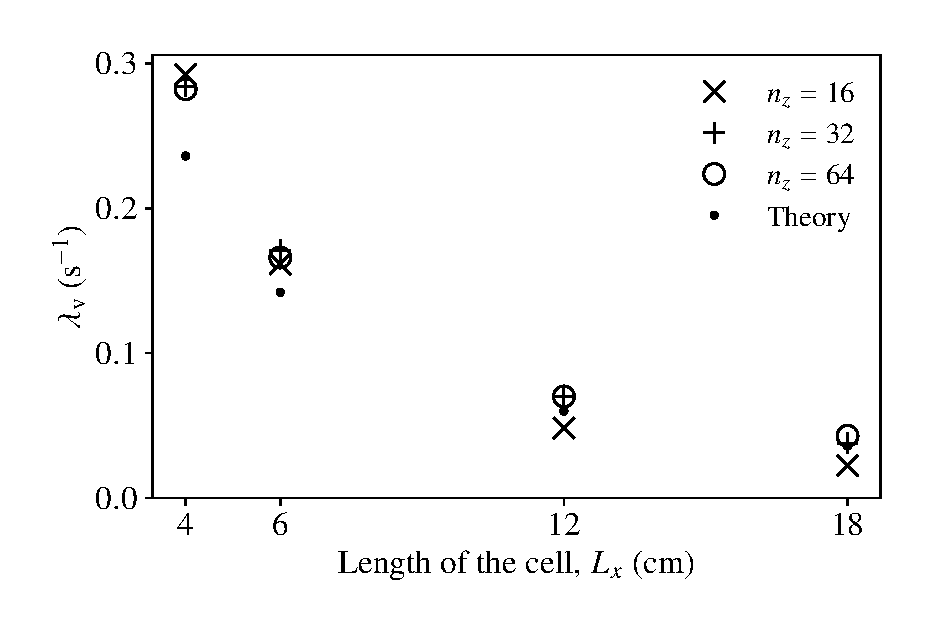
\includegraphics[height=5.5cm]{figures/AR_damp1_10.eps} };
		\node (pic2) at (4,0)
		{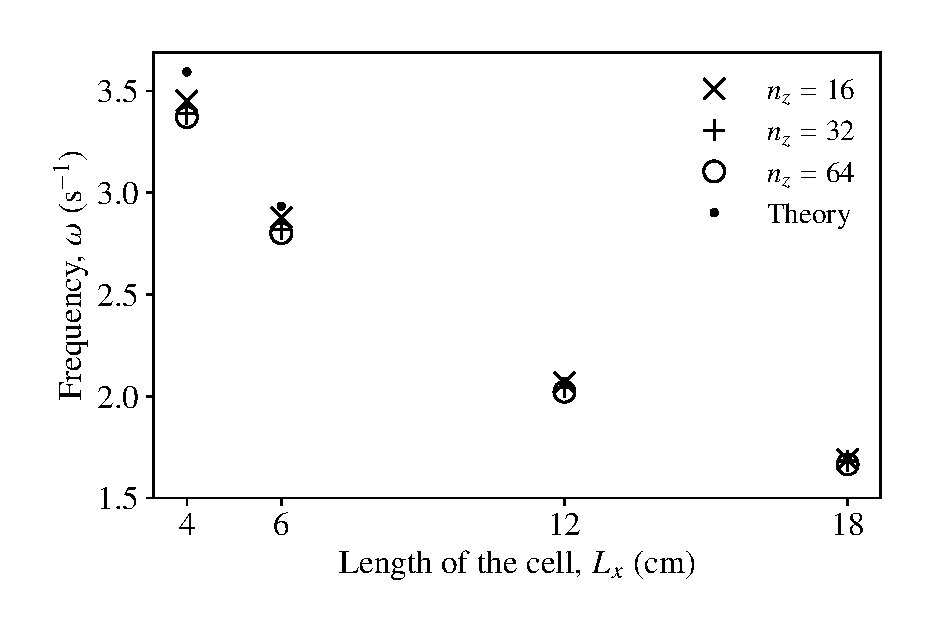
\includegraphics[height=5.5cm]{figures/AR_omega1_10.eps} };
		\node [above of=pic1, xshift=-3.5cm, yshift=1.9cm] {$(a)$};
		\node [above of=pic2, xshift=-3.2cm, yshift=1.9cm] {$(b)$};
		
		\node (pic3) at (-4,-5.7) 
		{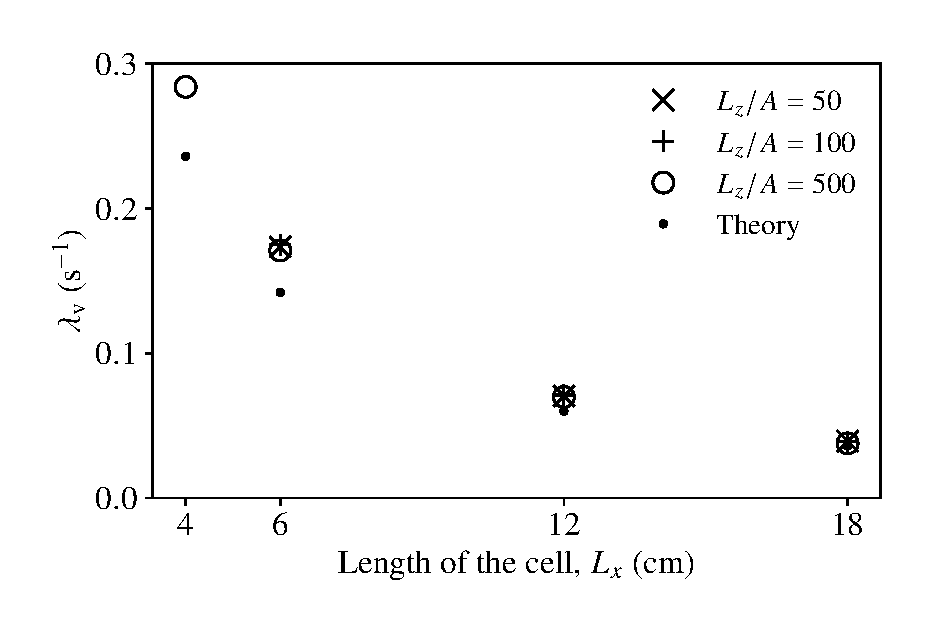
\includegraphics[height=5.5cm]{figures/AR_damp1_10_LyOA.eps} };
		\node (pic4) at (4,-5.7)
		{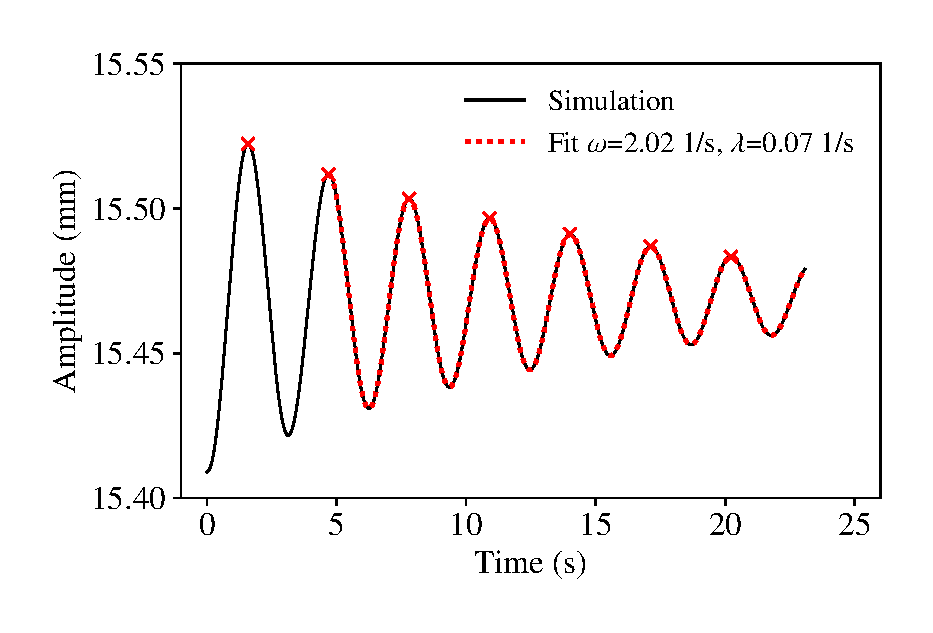
\includegraphics[height=5.5cm]{figures/AR1_10_Lx12cm_LyOA500_EE_ny64.eps} };
		\node [above of=pic1, xshift=-3.5cm, yshift=-3.8cm] {$(c)$};
		\node [above of=pic2, xshift=-3.2cm, yshift=-3.8cm] {$(d)$};
	\end{tikzpicture}
	\caption{The grid independence test observing the (a) viscous damping rate and (b) wave frequency for different cell sizes for aspect ratio 1 and wave number ($1,0$). (c) The same case was simulated with different initial wave amplitudes to certify the independence of initial wave amplitude on the damping rate. (d) the post-processing done on a cell size of $12\times 12\times 3$ cm, the resultant slope of the exponential curve fit of the amplitude signal at a local point $-L_x/2, -L_y/2$ to determine the wave frequency and the damping rate.}
	\label{fig:addn_detail}
\end{figure}
%%%%%%%%%%%%%%   

\begin{table}%[H] add [H] placement to break table across pages
	\caption{The detailed comparison of theoretical values of two-layer wave frequency and viscous damping with the numerical simulations of ARCHER code, for different cell dimensions and resultant wave modes. The two layers considered are cryolite and aluminum (see Table\,\ref{tab:table_properties}). The heights of the respective layers are equal i.e. $h_1=h_2$.}
	\label{tab:table_sim}
	\begin{ruledtabular}
		\begin{tabular}{lllllll}
			\multirow{2}{*}{Aspect ratio} &
			Cell dimensions, & \multirow{2}{*}{Wave mode (m,n)} &
			\multicolumn{2}{c}{Wave frequency $\omega$ (s\textsuperscript{-1})}
			& \multicolumn{2}{c}{Viscous damping rate $\lambda$ (s\textsuperscript{-1})} \\
			& $L_x \times L_y \times [h_1+h_2]$  (cm)	&   & Theory  & ARCHER & Theory  & ARCHER   \\
			\hline
			\multirow{4}{*}{1.0} & 4$\times$4$\times$1  & \multirow{4}{*}{(1,0)}           & 3.593 & 3.372 & 0.236   & $0.282$        \\
			&	6$\times$6$\times$1.5 &   & 
			2.934 & 2.801  & 0.142   & $0.166$        \\
			&	12$\times$12$\times$3 &   & 
			2.075 & 2.022  & 0.060    & $0.070$          \\
			&	18$\times$18$\times$4.5 &   & 
			1.694 & 1.666  & 0.036   & $0.043$       \\
			\hline
			\multirow{8}{*}{2.0} & \multirow{2}{*}{4$\times$2$\times$1} & (2,0) & 
			6.732 & 6.453 & 0.359   & 0.437          \\
			& & (1,1) & 
			7.383 & 7.078 & 0.403   & 0.504        \\
			\cline{2-7} 
			& \multirow{2}{*}{6$\times$3$\times$1.5}  & (2,0) & 
			5.496 & 5.357 & 0.216   & 0.260         \\
			& & (1,1) & 
			6.028 & 5.879 & 0.243   & 0.296         \\
			\cline{2-7} 
			& \multirow{2}{*}{12$\times$6$\times$3} & (2,0) & 
			3.887 & 3.858 & 0.090    & 0.095        \\
			& & (1,1) & 
			4.262 & 4.233 & 0.102   & 0.104      \\
			\cline{2-7} 
			& \multirow{2}{*}{18$\times$9$\times$4.5} & (2,0)  & 
			3.173 & 3.164 & 0.054   & 0.047         \\
			& & (1,1) & 
			3.480 & 3.471 & 0.061   & 0.051          \\
			\hline
			\multirow{16}{*}{3.0} & \multirow{4}{*}{4$\times$1.34$\times$1} & (3,0) &
			9.258 & 8.875 & 0.474   & 0.585         \\
			& & (0,1) & 
			9.258 & 8.929 & 0.435   & 0.527         \\
			& & (5,0) & 
			12.89 & 12.44 &0.644   & 0.819          \\
			& & (4,1) & 
			12.89 & 12.33 & 0.755   & 0.901         \\
			\cline{2-7} 
			& \multirow{4}{*}{6$\times$2$\times$1.5} & (3,0) & 
			7.559 & 7.347 & 0.285   & 0.347         \\
			& & (0,1) & 
			7.559 & 7.379 & 0.261   & 0.315         \\
			& & (5,0) & 
			10.52 & 10.28 & 0.385   & 0.485          \\
			& & (4,1) & 
			10.52 & 10.23 & 0.452   & 0.548        \\
			\cline{2-7} 
			& \multirow{4}{*}{12$\times$4$\times$3} & (3,0) & 
			5.345 & 5.288 & 0.119   & 0.137         \\
			& & (0,1) & 
			5.345 & 5.296 & 0.109   & 0.126         \\
			& & (5,0) & 
			7.440 & 7.384 & 0.161   & 0.177          \\
			& & (4,1) & 
			7.440 & 7.373 & 0.189   & 0.207         \\
			\cline{2-7} 
			& \multirow{4}{*}{18$\times$6$\times$4.5} & (3,0) & 
			4.364 & 4.343 & 0.072   & 0.073         \\
			& & (0,1) & 
			4.364 & 4.346 & 0.066   & 0.067         \\
			& & (5,0) & 
			6.075 & 6.054 & 0.097   & 0.089        \\
			& & (4,1) & 
			6.075 & 6.051 & 0.114   & 0.104          
		\end{tabular}
	\end{ruledtabular}
\end{table}



\clearpage
% If you have acknowledgments, this puts in the proper section head.
\begin{acknowledgments}
This study was supported by Deutsche Forschungsgemeinschaft (DFG, German Research Foundation) by Award No. 512131026. The authors report no conflict of interest. The author, Marie-Charlotte Renoult acknowledge the financial support provided by the French Agence Nationale de la Recherche (ANR) LaBEx EMC3 through the HILIMBA project (Grant No. 10-LABX-0009) for initiating the collaboration between HZDR and CORIA. The numerical work was granted access to the HPC resources of IDRIS, TGCC and CINES under the allocation A0132B1010 made by GENCI (Grand Equipement National de Calcul Intensif) and the CRIANN (Centre Régional Informatique et d’Applications Numériques de Normandie) under the scientific project N. 201 704. Lastly, the authors would like to thank William Nash for proofreading the manuscript.
\end{acknowledgments}

% Create the reference section using BibTeX:

\bibliography{prf}

\end{document}
%
% ****** End of file apstemplate.tex ******

